\documentclass[10pt]{article}

\usepackage{preprint}
\usepackage{amsmath}
\usepackage{graphicx}
\usepackage{booktabs}
\usepackage{tabularx}
\usepackage{array}
\usepackage{float}
% Floats stay in the section that discusses them (placeins), and try "here" first.
\usepackage[section]{placeins}
\usepackage[labelformat=parens,labelsep=space]{subcaption}
\usepackage{tikz}
\usetikzlibrary{arrows.meta,positioning,calc,fit,backgrounds}
\usepackage{pgfplots}
\pgfplotsset{compat=1.18}
\usepackage[numbers,sort&compress]{natbib}
\usepackage{hyperref}
\usepackage{url}
\usepackage{xurl}

\definecolor{linkblue}{RGB}{0,20,115}
\definecolor{urlmag}{RGB}{160,40,120}
\hypersetup{colorlinks=true,linkcolor=linkblue,citecolor=linkblue,urlcolor=urlmag}

% ------------------------------------------------------------------------------
% Palette: the app's tokens (docs/design-rules.md). Data colours are the chart colours.
% ------------------------------------------------------------------------------
\definecolor{ink}{HTML}{17181A}
\definecolor{ink2}{HTML}{5C5F66}
\definecolor{line}{HTML}{E6E5E1}
\definecolor{accent}{HTML}{1F6F8B}
\definecolor{accentsoft}{HTML}{E9F1F3}
\definecolor{ok}{HTML}{2E7D4F}
\definecolor{warn}{HTML}{B7791F}
\definecolor{fault}{HTML}{B3261E}
\definecolor{dblue}{HTML}{0072B2}
\definecolor{dorange}{HTML}{C65300}
\definecolor{dgreen}{HTML}{007A5E}
\definecolor{dgrey}{HTML}{5A5A5A}

\pgfplotsset{
  every axis/.append style={width=\linewidth, height=4.6cm, grid=major, grid style={line, line width=0.3pt},
    tick label style={font=\scriptsize}, label style={font=\scriptsize}, legend style={font=\scriptsize, draw=line, fill=white, fill opacity=0.9, text opacity=1},
    axis line style={ink2}, every axis plot/.append style={line width=0.9pt}},
}

\graphicspath{{./figures/}}
\newcommand{\sdv}{Duma~SDV}
% A car render from the stage, cropped to the car (1900 x 1440 px captures).
\newcommand{\carrender}[2]{\includegraphics[width=\linewidth, trim=#2, clip]{#1}}
% Table rows from a generated file: the primitive input is safe inside tabular.
\makeatletter\newcommand{\inputrows}[1]{\@@input #1 }\makeatother
% Generated by paper/data/export.ts. Do not edit.
\newcommand{\ParMotorKw}{230}
\newcommand{\ParMotorNm}{360}
\newcommand{\ParRatio}{10.81}
\newcommand{\ParPackKwh}{82.5}
\newcommand{\ParPackV}{550}
\newcommand{\ParCells}{172}
\newcommand{\ParTestMass}{2130}
\newcommand{\ParCd}{0.22}
\newcommand{\ParArea}{2.35}
\newcommand{\ParCrr}{0.0110}
\newcommand{\ParObcKw}{11}
\newcommand{\ParDcKw}{150}
\newcommand{\ParPrechargeOhm}{200}
\newcommand{\ParDcLinkMf}{1.0}
\newcommand{\ParTickMs}{10}
\newcommand{\StartWakeMs}{310}
\newcommand{\StartSelfCheckMs}{510}
\newcommand{\StartPrechargeMs}{1310}
\newcommand{\StartContactorsMs}{1610}
\newcommand{\StartReadyMs}{1620}
\newcommand{\StartReadyS}{1.62}
\newcommand{\StartBootFrames}{5}
\newcommand{\ResZeroHundred}{5.97}
\newcommand{\ResRange}{498}
\newcommand{\ResRangeWhKm}{165.6}
\newcommand{\ResAnchorWhKm}{180.1}
\newcommand{\ResDcMin}{34.0}
\newcommand{\ResDcPeakKw}{150}
\newcommand{\ResAcHours}{6.13}
\newcommand{\ResRegenKineticKj}{824}
\newcommand{\ResRegenPackKj}{552}
\newcommand{\ResRegenShare}{67}
\newcommand{\ResRegenRecoveredWh}{153}
\newcommand{\ResRegenLiftS}{4}
\newcommand{\ResRegenBrakeS}{8.0}
\newcommand{\ResRegenSpeedKmh}{100}
\newcommand{\ResRegenPeakKw}{56}
\newcommand{\ResRegenAllowKw}{60}
\newcommand{\ResRegenSocPct}{80}
\newcommand{\CycUrbanKm}{3.10}
\newcommand{\CycUrbanKwh}{0.449}
\newcommand{\CycUrbanDurS}{589}
\newcommand{\CycUrbanMotorMaxC}{31.1}
\newcommand{\CycUrbanPackMaxC}{23.0}
\newcommand{\CycUrbanEco}{146.4}
\newcommand{\CycUrbanNormal}{144.8}
\newcommand{\CycUrbanSport}{144.8}
\newcommand{\CycHighwayKm}{8.26}
\newcommand{\CycHighwayKwh}{1.512}
\newcommand{\CycHighwayDurS}{322}
\newcommand{\CycHighwayMotorMaxC}{39.3}
\newcommand{\CycHighwayPackMaxC}{23.1}
\newcommand{\CycHighwayEco}{183.3}
\newcommand{\CycHighwayNormal}{183.2}
\newcommand{\CycHighwaySport}{183.2}
\newcommand{\FaultDtcMs}{60}
\newcommand{\FaultLimitMs}{60}
\newcommand{\FaultLimitKw}{128}
\newcommand{\FaultDecisionMs}{160}
\newcommand{\FaultWarningMs}{80}
\newcommand{\FaultCompareS}{4.5}
\newcommand{\FaultHealthyKw}{251}
\newcommand{\FaultDeratedKw}{127}
\newcommand{\FaultCount}{4}
\newcommand{\OtaCheckS}{1.0}
\newcommand{\OtaDownloadS}{7.0}
\newcommand{\OtaVerifyS}{8.0}
\newcommand{\OtaInstallStartS}{8.0}
\newcommand{\OtaRebootS}{13.0}
\newcommand{\OtaOffS}{13.1}
\newcommand{\OtaInstalledS}{13.4}
\newcommand{\OtaReadyS}{14.8}
\newcommand{\OtaRestartS}{1.8}
\newcommand{\OtaSizeMb}{48}
\newcommand{\OtaRateMbs}{8}
\newcommand{\OtaVersion}{1.1.0}
\newcommand{\OtaBootVersion}{1.1.0}
\newcommand{\BusFramesPerS}{500}
\newcommand{\BusMessages}{23}
\newcommand{\BusPeriodic}{18}
\newcommand{\BusNodes}{6}
\newcommand{\BusSignals}{61}


\title{\sdv: A Browser-Based Digital Twin of a Software-Defined Electric Vehicle}
\author{FNM}
\affiliation{Software-Defined Electric Vehicle Design Challenge}

\begin{document}

\maketitle

\begin{abstract}
A software-defined vehicle (SDV) is a car whose behaviour is decided, and can be changed, by software. Its design is hard to judge from diagrams alone, because the interesting part is how the software modules coordinate. We present \sdv{}, a digital twin of a fictional rear-drive electric sedan that runs in a web browser, online or fully offline. Six electronic control units (ECUs) are separate software modules that exchange only messages on a simulated CAN bus: a vehicle control unit, battery management, motor control, an on-board charger, an instrument cluster and a telematics unit. They sit on physical plant models of the vehicle, battery, high-voltage circuit and thermal masses, advanced in deterministic \ParTickMs\,ms steps. A judge can power the car on, drive it, charge it on AC or DC, inject faults and install an over-the-air (OTA) update, while a 3D model, a driver dashboard and a live bus trace show every step. Automated tests hold the physics to the published figures of a production reference car: 0--100\,km/h in \ResZeroHundred\,s (target 5.9\,s), \ResRange\,km at a steady 100\,km/h (510\,km) and \ResDcMin\,min for a 10--80\,\% DC charge (37\,min), all within the $\pm 10\,\%$ goal. Under a cell over-temperature fault the battery management unit halves its discharge allowance within \FaultLimitMs\,ms and the drive power follows it. The OTA update downloads, verifies and installs into an inactive firmware bank, restarts the car and unlocks a drive mode in \OtaReadyS\,s. Every figure in this paper is generated from the simulator.
\end{abstract}

% ==============================================================================
\section{Introduction}
% ==============================================================================

An electric vehicle is increasingly a software product. Its supervisor decides how pedal travel becomes torque, when the high-voltage (HV) battery may connect, how braking is shared between the motor and the friction brakes, and how the car responds when a sensor reports a fault~\cite{ehsani2018}. In a software-defined vehicle these decisions live in updatable software on a network of electronic control units (ECUs), and an over-the-air update can change the car after it is sold~\cite{unece_r156}.

A design challenge for such a vehicle asks for its software ecosystem without a physical car. The usual answer is an architecture diagram and a mock-up screen. Judges then have to take on trust that the modules would work together: they cannot watch a fault spread from a sensor to a warning light, or see a software update change how the car drives.

\sdv{} makes the design something a judge can run and check. It is a digital twin~\cite{grieves2017} in the practical sense: a model of the vehicle and of its software that behaves like the real system under the same inputs. Our contributions are:
\begin{itemize}
  \item An ECU architecture in which every module is separate code that knows other modules \textbf{only through CAN messages} declared once in a catalogue. The architecture view and the tables in this paper are drawn from that catalogue, so the diagram cannot disagree with the code.
  \item A \textbf{deterministic, framework-free simulation core} that runs the same code headlessly in tests and behind a 60\,fps browser view.
  \item Physics calibrated to a published reference car and \textbf{held within $\pm 10\,\%$} by automated tests.
  \item Complete software flows for \textbf{startup, driving, regenerative braking, AC and DC charging, fault diagnosis and OTA update}, each playable from a one-button guided demo and each verified by an end-to-end browser test.
\end{itemize}

\begin{figure}[!htbp]
\centering
\begin{subfigure}[t]{0.325\textwidth}\centering
\carrender{car-front}{120 330 120 380}
\caption{Front three-quarter.}
\end{subfigure}\hfill
\begin{subfigure}[t]{0.325\textwidth}\centering
\carrender{car-side}{120 400 120 420}
\caption{Side.}
\end{subfigure}\hfill
\begin{subfigure}[t]{0.325\textwidth}\centering
\carrender{car-rear}{120 330 120 380}
\caption{Rear three-quarter.}
\end{subfigure}
\caption{\textbf{The \sdv{} car on the app's 3D stage.} A smooth, stylised fastback built in code at the reference car's size, with no branding. These are screen captures of the running app (three.js), not offline renders.}
\label{fig:car}
\end{figure}

% ==============================================================================
\section{Requirements and scope}
% ==============================================================================

The competition names five required scenarios; we add the OTA update as a sixth (Table~\ref{tab:scenarios}). Each must run unaided in under a minute from the first click, from a public link and from a laptop with no network. The ranked trade-offs that decide conflicts are, in order: correctness of the physics and engineering, demo reliability, user experience, performance, code simplicity and delivery speed.

\begin{table}[!htbp]
\caption{\textbf{Scenarios and where they are verified.} Every scenario is scripted in the guided demo and has its own browser test that plays it from the demo.}
\label{tab:scenarios}
\centering\small
\begin{tabularx}{\textwidth}{@{}lXl@{}}
\toprule
Scenario & What the judge sees & Key ECUs \\
\midrule
Startup & 12\,V wake, self-checks, pre-charge, contactors, READY; boot frames on the bus & VCU, BMS, MCU \\
Driving & Pedal to torque request, speed, power, SOC and range on the dashboard & VCU, MCU, IC \\
Regen & Negative power on lift-off, blended braking, energy recovered & VCU, MCU, BMS \\
Charging & AC through the on-board charger, DC around it; charge curve and time to target & VCU, BMS, OBC \\
Fault & DTC on the bus, derate or limp mode, plain-language warning, highlighted module & BMS, MCU, VCU, IC \\
OTA update & Check, download, verify, install, restart; a new drive mode appears & TCU, VCU \\
\bottomrule
\end{tabularx}
\end{table}

Out of scope are real hardware, autonomous driving, any backend, and an open road network: the car drives on a rolling-road stage. The vehicle is fictional. It takes its specifications from a production mid-size rear-drive sedan with a lithium iron phosphate (LFP) pack, which we call the \emph{reference car} and never name.

% ==============================================================================
\section{System architecture}
% ==============================================================================

\subsection{Layers}

The application has three layers (Figure~\ref{fig:layers}). The \emph{simulation core} is plain TypeScript with no user-interface, 3D or browser dependencies; a lint rule rejects imports of React or three.js, the wall clock and unseeded random numbers. The \emph{stores} hold the current simulation and the user-interface state. The \emph{views} and the 3D stage only read snapshots and send inputs. A frame loop converts wall time into a whole number of simulation steps, scaled by a user-selectable time scale of 1$\times$ to 120$\times$, so a 35-minute charge can be watched in seconds.

\begin{figure}[!htbp]
\centering
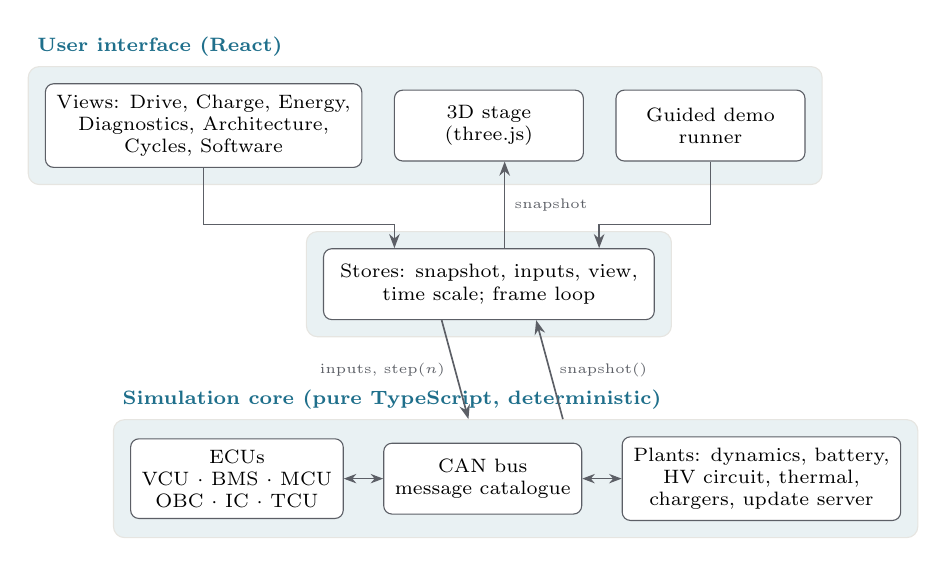
\begin{tikzpicture}[
  box/.style={draw=ink2, rounded corners=3pt, fill=white, align=center, font=\scriptsize, inner sep=4pt, minimum height=0.9cm},
  layer/.style={draw=line, rounded corners=4pt, fill=accentsoft, inner sep=6pt},
  lab/.style={font=\scriptsize\bfseries, text=accent, anchor=north west},
  arr/.style={-{Stealth[length=1.8mm]}, draw=ink2, line width=0.6pt},
]
\node[box, minimum width=3.6cm] (views) at (0,0) {Views: Drive, Charge, Energy,\\Diagnostics, Architecture,\\Cycles, Software};
\node[box, minimum width=2.4cm, right=0.4cm of views] (stage) {3D stage\\(three.js)};
\node[box, minimum width=2.4cm, right=0.4cm of stage] (demo) {Guided demo\\runner};
\node[box, minimum width=4.2cm, below=1.1cm of stage] (store) {Stores: snapshot, inputs, view,\\time scale; frame loop};
\node[box, minimum width=2.6cm, below=1.5cm of store, xshift=-3.2cm] (ecus) {ECUs\\VCU $\cdot$ BMS $\cdot$ MCU\\OBC $\cdot$ IC $\cdot$ TCU};
\node[box, minimum width=2.2cm, right=0.5cm of ecus] (bus) {CAN bus\\message catalogue};
\node[box, minimum width=3.0cm, right=0.5cm of bus] (plant) {Plants: dynamics, battery,\\HV circuit, thermal,\\chargers, update server};
\begin{scope}[on background layer]
\node[layer, fit=(views)(stage)(demo)] (ui) {};
\node[layer, fit=(store)] (st) {};
\node[layer, fit=(ecus)(bus)(plant)] (core) {};
\end{scope}
\node[lab, anchor=south west] at (ui.north west) {User interface (React)};
\node[lab, anchor=south west] at (core.north west) {Simulation core (pure TypeScript, deterministic)};
\draw[arr] (views.south) |- ($(store.north)+(-1.2,0.3)$) -- ++(0,-0.3);
\draw[arr] ($(store.north)+(0.2,0)$) -- node[right, font=\tiny, text=ink2] {snapshot} ($(stage.south)+(0.2,0)$);
\draw[arr] (demo.south) |- ($(store.north)+(1.4,0.3)$) -- ++(0,-0.3);
\draw[arr] ($(store.south)+(-0.6,0)$) -- node[left, font=\tiny, text=ink2] {inputs, step($n$)} ($(core.north)+(-0.6,0)$);
\draw[arr] ($(core.north)+(0.6,0)$) -- node[right, font=\tiny, text=ink2] {snapshot()} ($(store.south)+(0.6,0)$);
\draw[{Stealth[length=1.6mm]}-{Stealth[length=1.6mm]}, draw=ink2] (ecus) -- (bus);
\draw[{Stealth[length=1.6mm]}-{Stealth[length=1.6mm]}, draw=ink2] (bus) -- (plant);
\end{tikzpicture}
\caption{\textbf{Layers.} The simulation core has no user-interface or browser dependencies. The views, the 3D stage and the guided demo drive it only through inputs and read it only through snapshots.}
\label{fig:layers}
\end{figure}

\subsection{ECUs and the bus}

The core separates two kinds of model. \emph{Plants} are the physical world: longitudinal vehicle dynamics, the pack's open-circuit voltage and internal resistance, the HV circuit with its contactors and DC-link capacitor, lumped thermal masses with two coolant loops~\cite{pesaran2002}, the AC wallbox, the DC charger and the update server. \emph{ECUs} are software. An ECU senses its own plant signals (the BMS its cell temperatures, the MCU its DC-link voltage and rotor speed) and learns everything else from bus messages. No ECU reads another ECU's state directly. This rule is what makes the architecture view truthful: if a signal matters to an ECU, it appears on the bus trace.

\begin{figure}[!htbp]
\centering
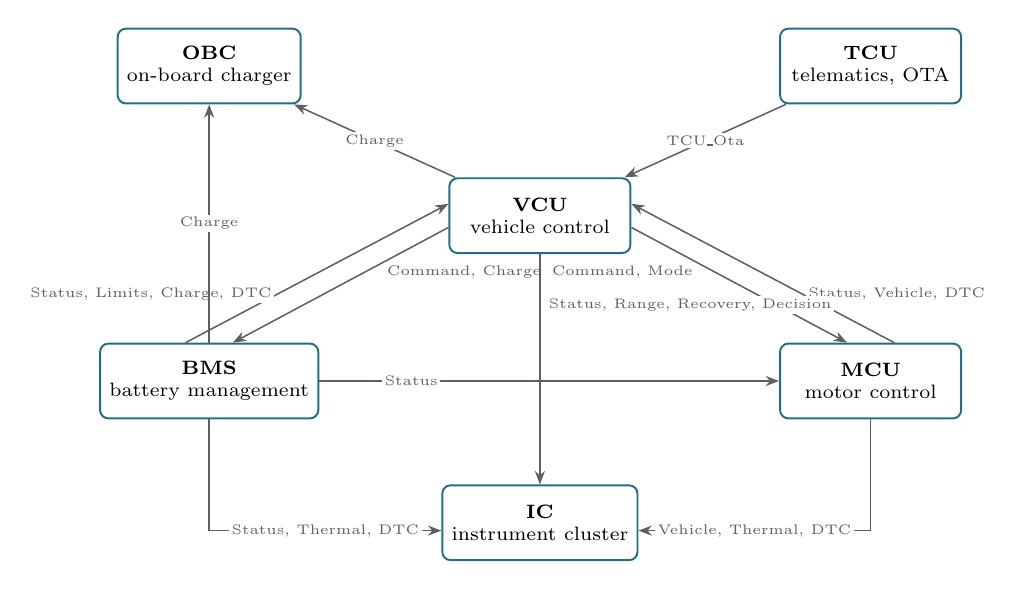
\begin{tikzpicture}[
  ecu/.style={draw=accent, rounded corners=3pt, fill=white, align=center, font=\scriptsize, minimum width=2.3cm, minimum height=0.95cm, line width=0.7pt},
  msg/.style={-{Stealth[length=1.7mm]}, draw=ink2, line width=0.55pt},
  lbl/.style={font=\tiny, text=ink2, fill=white, inner sep=1pt},
]
\node[ecu] (vcu) at (0,0) {\textbf{VCU}\\vehicle control};
\node[ecu] (bms) at (-4.2,-2.1) {\textbf{BMS}\\battery management};
\node[ecu] (mcu) at (4.2,-2.1) {\textbf{MCU}\\motor control};
\node[ecu] (obc) at (-4.2,1.9) {\textbf{OBC}\\on-board charger};
\node[ecu] (ic) at (0,-3.9) {\textbf{IC}\\instrument cluster};
\node[ecu] (tcu) at (4.2,1.9) {\textbf{TCU}\\telematics, OTA};
\draw[msg] ($(vcu.west)+(0,-0.15)$) -- node[lbl, pos=0.3, below right=0pt] {Command, Charge} ($(bms.north)+(0.3,0)$);
\draw[msg] ($(bms.north)+(-0.3,0)$) -- node[lbl, pos=0.35, left=1pt] {Status, Limits, Charge, DTC} ($(vcu.west)+(0,0.15)$);
\draw[msg] ($(vcu.east)+(0,-0.15)$) -- node[lbl, pos=0.3, below left=0pt] {Command, Mode} ($(mcu.north)+(-0.3,0)$);
\draw[msg] ($(mcu.north)+(0.3,0)$) -- node[lbl, pos=0.35, right=1pt] {Status, Vehicle, DTC} ($(vcu.east)+(0,0.15)$);
\draw[msg] (vcu) -- node[lbl] {Charge} (obc);
\draw[msg] (bms) -- node[lbl] {Charge} (obc);
\draw[msg] (tcu) -- node[lbl] {TCU\_Ota} (vcu);
\draw[msg] (bms.south) |- node[lbl, pos=0.75] {Status, Thermal, DTC} ($(ic.west)+(0,-0.1)$);
\draw[msg] (mcu.south) |- node[lbl, pos=0.75] {Vehicle, Thermal, DTC} ($(ic.east)+(0,-0.1)$);
\draw[msg] (vcu) -- node[lbl, pos=0.22, right=2pt] {Status, Range, Recovery, Decision} (ic);
\draw[msg] (bms) -- node[lbl, pos=0.2] {Status} (mcu);
\end{tikzpicture}
\caption{\textbf{ECUs and their main messages.} Arrows run from sender to subscriber; message names omit the sender prefix (\texttt{BMS\_Status} appears as Status beside the BMS). The TCU also subscribes to boot, status, charge, speed and SOC frames to check the install preconditions. The OBC only listens. The full catalogue is Table~\ref{tab:catalogue}.}
\label{fig:ecus}
\end{figure}

Figure~\ref{fig:ecus} shows the six ECUs. The \textbf{VCU} is the supervisor: it senses the power button, pedals and gear selector, owns the switched 12\,V supply of the other ECUs, runs the power state machine and the startup sequence, applies the gear interlocks, turns pedal travel into a torque request, decides derates, and estimates range. The \textbf{BMS} estimates state of charge (SOC), monitors cell temperature, controls the contactors and pre-charge, and publishes the charge and discharge limits. The \textbf{MCU} turns torque requests into motor torque within the motor envelope, and only while the VCU commands READY, the BMS reports closed contactors and the DC link it measures is charged. The \textbf{OBC} converts AC for the pack when the VCU and BMS both authorise it. The \textbf{IC} builds the dashboard, including its warnings, only from frames it receives, and marks a value unavailable when its frame goes stale. The \textbf{TCU} is the car's link to the update server and runs the OTA client.

\subsection{Message catalogue}

Every message is declared once, with its identifier, sender, period and signals with units and scaling (Table~\ref{tab:catalogue}). The bus delivers frames sent in one step at the start of the next, so every hop costs at least one step, and a frame older than two or three periods counts as lost. The catalogue has \BusMessages{} messages (\BusPeriodic{} periodic, from 10\,ms to 1\,s, and \StartBootFrames{} event-driven boot frames that carry each ECU's self-check result and software version) with \BusSignals{} signals among \BusNodes{} nodes. While driving the bus carries \BusFramesPerS{} frames per second. Identifiers group by sender: \texttt{0x1xx} VCU, \texttt{0x2xx} BMS, \texttt{0x3xx} MCU, \texttt{0x4xx} TCU. The bus models message timing and loss, not bit timing or arbitration~\cite{iso11898}. The Architecture view (Figure~\ref{fig:archview}) draws the same topology live, marks which ECUs are transmitting, and lists every frame in a trace that can be filtered by ECU or message and paused.

\begin{table}[!htbp]
\caption{\textbf{Message catalogue}, generated from the code. Period in ms; subscribers from the live topology.}
\label{tab:catalogue}
\centering\scriptsize
\begin{tabular}{@{}llrrl@{}}
\toprule
ID & Message & Period & Signals & Subscribers \\
\midrule
\inputrows{data/catalogue.tex}
\bottomrule
\end{tabular}
\end{table}

\begin{figure}[!htbp]
\centering
\begin{minipage}[c]{0.3\textwidth}\centering
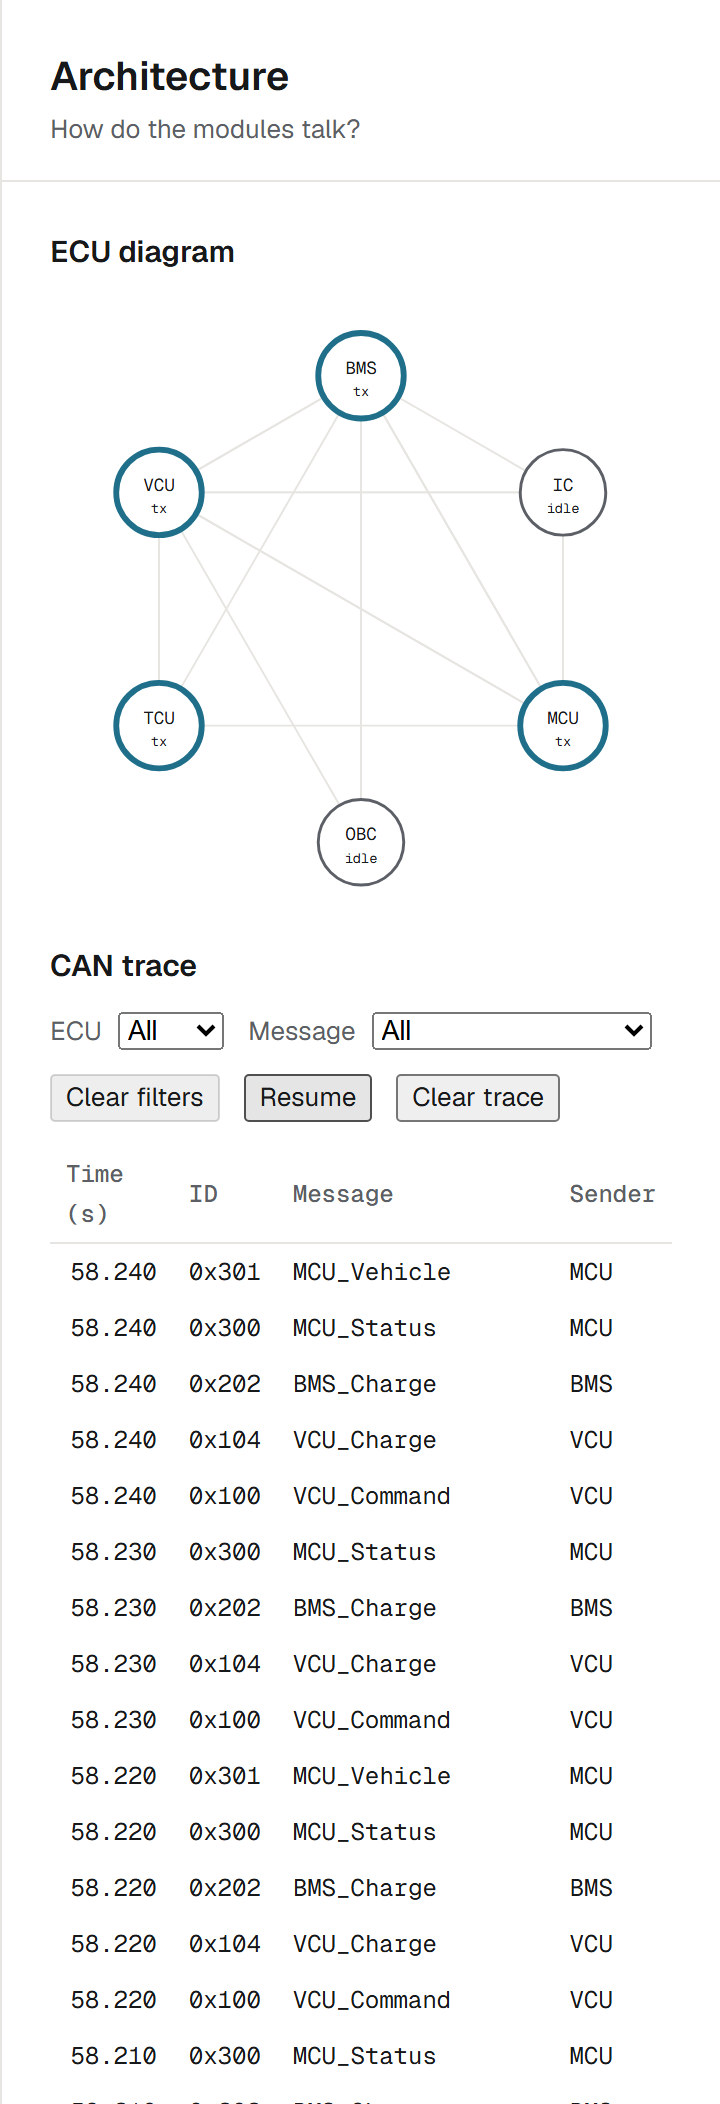
\includegraphics[width=\linewidth, trim=0 700 0 0, clip]{ui-architecture-panel}
\end{minipage}\hfill
\begin{minipage}[c]{0.66\textwidth}
\caption{\textbf{The Architecture view while driving}, paused. The ECU diagram is built from the live bus topology; a node reads \emph{tx} while it transmits and \emph{idle} otherwise (the OBC only listens, the IC's frames are all received). Below it, the CAN trace lists frames with sim time, identifier, name and sender; selecting one shows its decoded signals.}
\label{fig:archview}
\end{minipage}
\end{figure}

% ==============================================================================
\section{Software design}
% ==============================================================================

\subsection{A deterministic core}

The simulation advances in fixed \ParTickMs\,ms steps (100\,Hz). SI units are used throughout the core, and km/h, kW and kWh appear only at the user-interface boundary. The same initial state and input sequence always give identical snapshots and bus traces; tests check this for startup, driving, charging and the fault flow. Determinism lets a test drive the car through a 30-hour range run or a 35-minute charge in seconds, and it lets the guided demo and the browser tests replay exactly what a judge would see.

\subsection{Power states and startup}

The VCU runs the power state machine OFF $\to$ ACCESSORY $\to$ STARTING $\to$ READY, with CHARGING while an authorised session runs. Startup has five steps (Figure~\ref{fig:startup}). On \emph{wake} the VCU switches on the 12\,V supply of the other ECUs and waits for their boot frames. In the \emph{self-check} it requires three consecutive plausible \texttt{BMS\_Status} frames with open contactors, fresh limit and fault frames, and the MCU in standby. \emph{Pre-charge} closes the negative and pre-charge contactors so the DC-link capacitance (\ParDcLinkMf\,mF) charges through \ParPrechargeOhm\,$\Omega$; the BMS reports done at 95\,\% of pack voltage. The main contactor then closes, and \emph{READY} follows once the MCU confirms that the DC link it measures is within 10\,\% of pack voltage. Each step has a timeout, and a failed step powers the car down with a reason. The car reaches READY \StartReadyS\,s after Power on.

\begin{figure}[!htbp]
\centering
\begin{tikzpicture}
\begin{axis}[xlabel={Time after Power on (ms)}, ylabel={Voltage (V)}, xmin=0, xmax=1800, ymin=0, ymax=650, legend pos=south east]
\addplot[dblue] table[x=t_ms, y=dclink_v, col sep=comma] {data/startup.csv};
\addplot[dgrey, dashed] table[x=t_ms, y=pack_v, col sep=comma] {data/startup.csv};
\legend{DC-link voltage (MCU side), pack terminal voltage}
\draw[accent, densely dotted] (axis cs:\StartWakeMs,0) -- (axis cs:\StartWakeMs,650) node[pos=0.97, anchor=south east, rotate=90, font=\tiny, text=accent] {wake};
\draw[accent, densely dotted] (axis cs:\StartSelfCheckMs,0) -- (axis cs:\StartSelfCheckMs,650) node[pos=0.97, anchor=south east, rotate=90, font=\tiny, text=accent] {self-check};
\draw[accent, densely dotted] (axis cs:\StartPrechargeMs,0) -- (axis cs:\StartPrechargeMs,650) node[pos=0.97, anchor=south east, rotate=90, font=\tiny, text=accent] {pre-charge};
\draw[accent, densely dotted] (axis cs:\StartContactorsMs,0) -- (axis cs:\StartContactorsMs,650) node[pos=0.97, anchor=south east, rotate=90, font=\tiny, text=accent] {contactors};
\end{axis}
\end{tikzpicture}
\caption{\textbf{Startup on the HV circuit.} Dotted lines mark the end of each step. The DC link charges through the pre-charge resistor, the main contactor closes onto a charged capacitor, and READY follows \StartReadyS\,s after Power on.}
\label{fig:startup}
\end{figure}

\subsection{Torque path and drive modes}

The VCU turns the accelerator into a torque request: pedal travel raised to a mode exponent, times the torque the motor can make at its current speed. It then applies three limits. The BMS discharge limit bounds \emph{battery} power, so the VCU solves for the largest torque whose shaft power plus modelled motor and inverter loss plus the auxiliary load stays within it. The VCU's own derate caps shaft power and speed when a fault calls for it. A limiter fades torque out over the last 2\,km/h below the speed limit. The MCU clamps the request to the motor envelope once more. Three drive modes change the maps (Table~\ref{tab:modes}); a mode change blends the old map into the new over 0.5\,s so the torque never steps.

\begin{table}[!htbp]
\caption{\textbf{Drive modes.} Values other than the motor limits are our estimates; Sport arrives with VCU software \OtaVersion{} (Section~\ref{sec:ota}). Energy on the WLTC phases~\cite{unece_gtr15}, measured at the pack terminals.}
\label{tab:modes}
\centering\small
\begin{tabular}{@{}lrrr@{}}
\toprule
 & Eco & Normal & Sport \\
\midrule
Pedal exponent & 1.6 & 1.0 & 0.8 \\
Shaft power cap (kW) & 140 & \ParMotorKw & \ParMotorKw \\
Lift-off regen deceleration ($g$) & 0.20 & 0.15 & 0.15 \\
Urban (Low phase, Wh/km) & \CycUrbanEco & \CycUrbanNormal & \CycUrbanSport \\
Highway (Extra High phase, Wh/km) & \CycHighwayEco & \CycHighwayNormal & \CycHighwaySport \\
\bottomrule
\end{tabular}
\end{table}

\subsection{Regenerative braking}

On lift-off the VCU requests generator torque for 0.15\,$g$ in Normal, faded in between 0.5 and 5\,m/s so the car does not creep backwards. The brake pedal can ask for up to 0.30\,$g$ of electric braking. Friction brakes fill whatever the pedal demands beyond the torque the MCU actually produces, so the driver's deceleration never depends on the battery's willingness to accept charge. Regen is refused when the BMS reports no charge allowance or a fault disables it, and the friction brakes then take the whole demand.

\subsection{Charging}

Plugging in requires P and a stopped car. The VCU and the BMS each authorise a session on their own charge messages, and the charger delivers current only while both frames are fresh and positive. AC passes through the on-board charger (\ParObcKw\,kW); DC goes around it to the pack, following a taper from the charger's \ParDcKw\,kW peak and the BMS allowance. The protocol with the charger itself~\cite{iso15118} is outside the model.

\subsection{Faults and safe states}
\label{sec:faults}

Four faults can be injected (Table~\ref{tab:faults}). The owning ECU raises a diagnostic trouble code (DTC) with an active or stored status in a bit field on its DTC message~\cite{iso14229}. The VCU combines the DTC frames into one drive decision, which the IC turns into a plain-language warning with an icon and the affected module; the 3D car highlights that module. Clearing the stored records asks for confirmation (Figure~\ref{fig:xray}). The responses follow the usual pattern of reducing capability to reach a safe state rather than stopping outright~\cite{iso26262}, but the model is not a safety analysis.

\begin{table}[!htbp]
\caption{\textbf{Fault catalogue and the car's response.}}
\label{tab:faults}
\centering\small
\begin{tabularx}{\textwidth}{@{}llllX@{}}
\toprule
Fault & DTC & Owner & Warning & Response \\
\midrule
Cell over-temperature & P0A7E & BMS & amber & Discharge allowance halved, charging and regen refused \\
Insulation fault & P0AA6 & BMS & red & No drive torque, startup and charging refused \\
Motor over-temperature & P0A2F & MCU & amber & Limp mode: 30\,kW, 50\,km/h, no regen \\
12\,V low & P0562 & VCU & amber & Limp mode: 20\,kW, 40\,km/h; startup refused \\
\bottomrule
\end{tabularx}
\end{table}

\begin{figure}[!htbp]
\centering
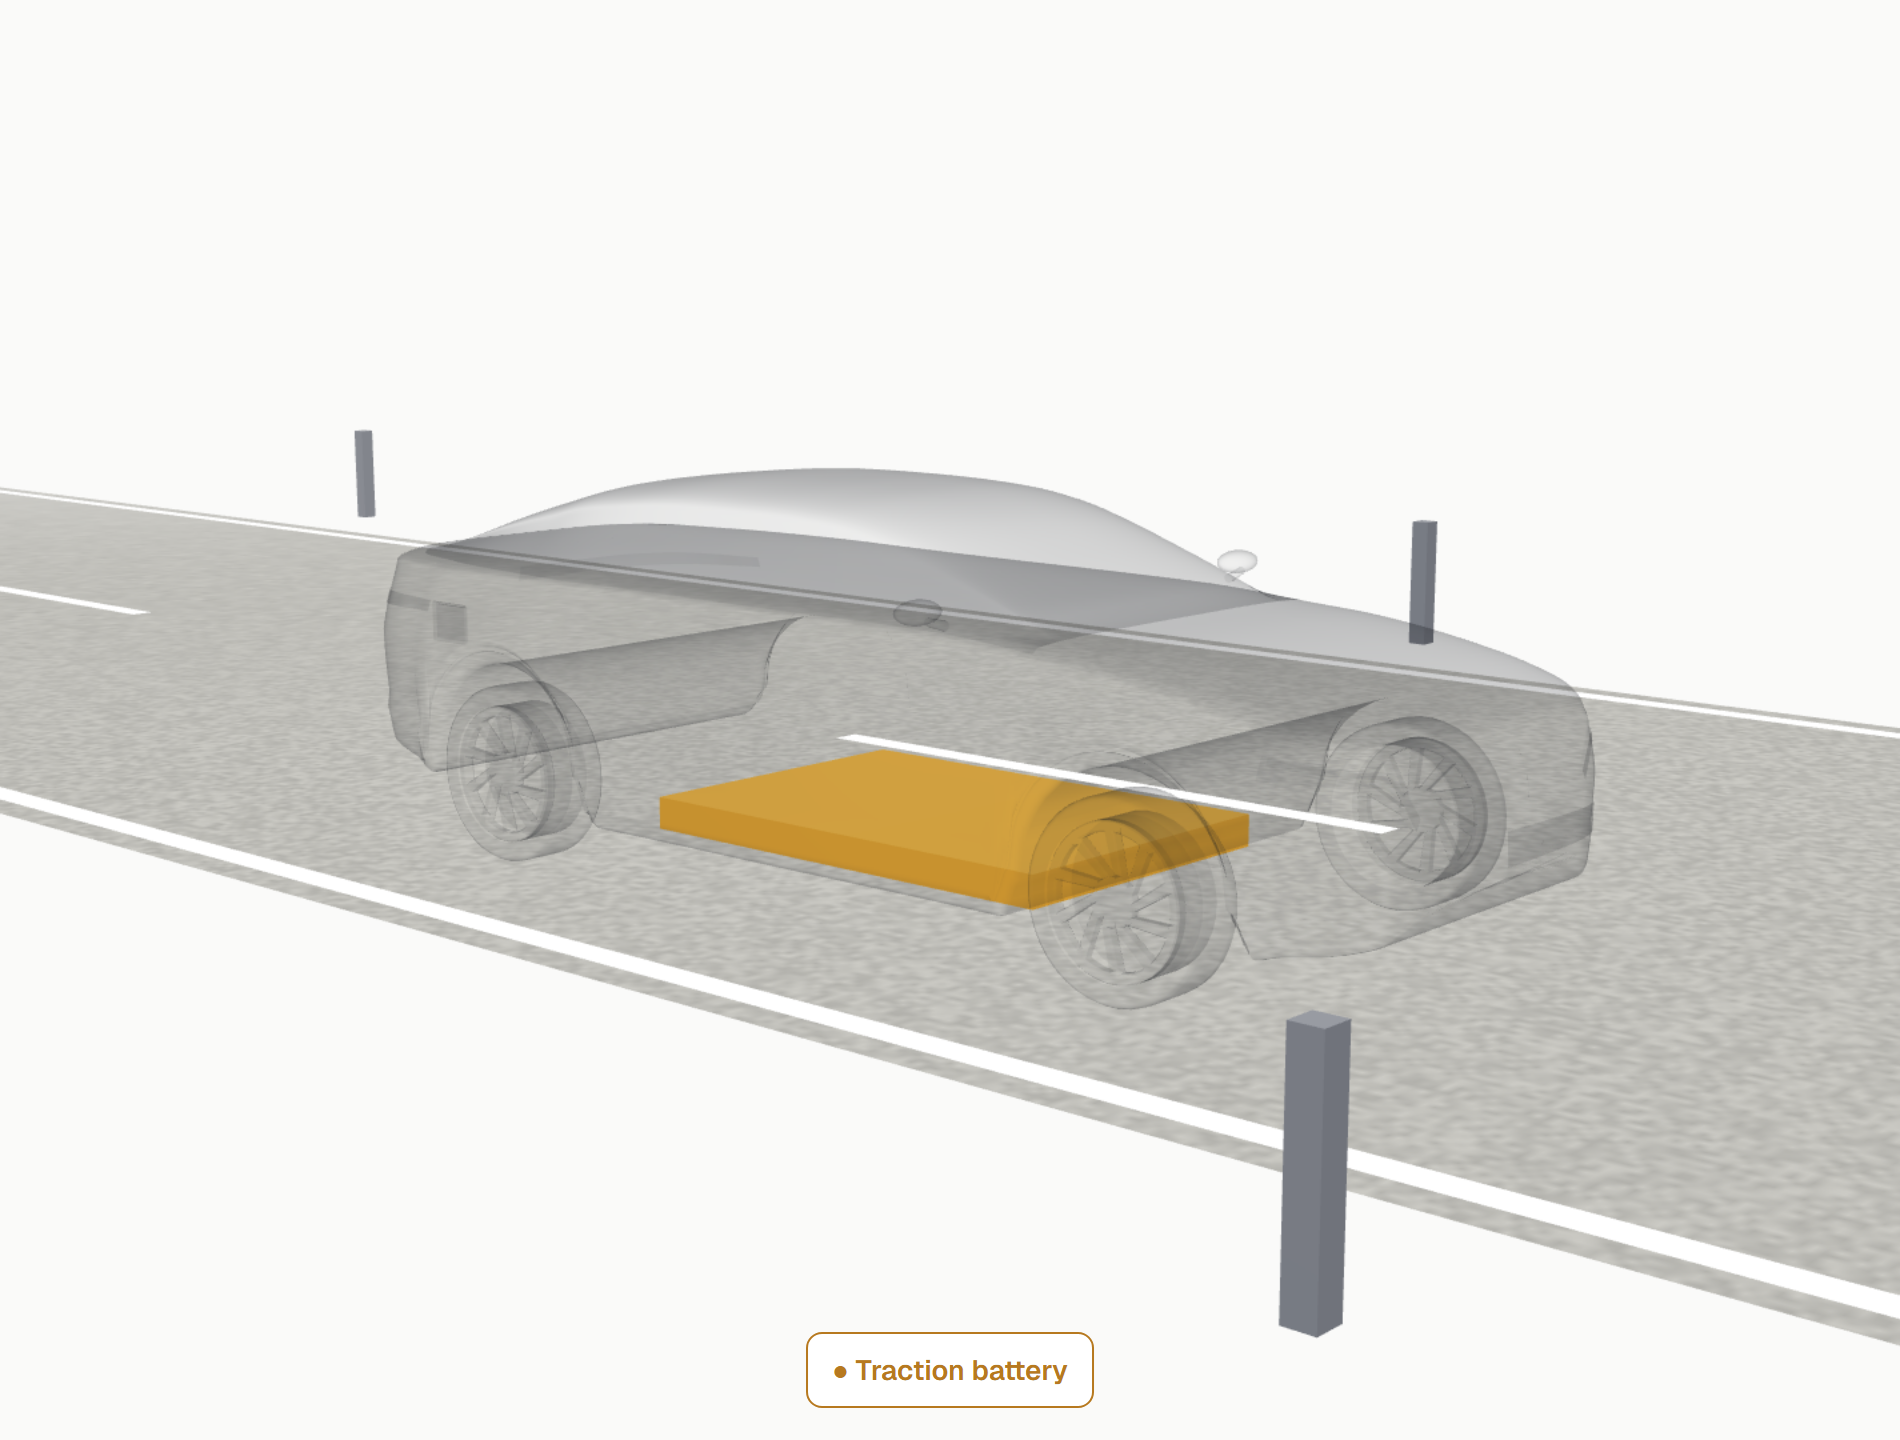
\includegraphics[width=0.62\textwidth, trim=0 20 0 380, clip]{car-xray}
\caption{\textbf{X-ray view during a cell over-temperature fault while driving.} The body turns translucent and the faulted module, the traction battery in the floor, glows in the warning colour, with its name in words so the status never relies on colour alone.}
\label{fig:xray}
\end{figure}

\subsection{Over-the-air update}
\label{sec:ota}

The OTA flow follows the structure of a managed software update~\cite{unece_r156}. The TCU checks the server, downloads a \OtaSizeMb\,MB VCU image at \OtaRateMbs\,MB/s (driving is allowed meanwhile), and verifies its signature and digest. It installs only when the driver confirms and the car is READY, in P, stopped, not charging and above 20\,\% SOC, all read from bus frames. The VCU holds two firmware banks. The image is written to the inactive bank while the running firmware keeps working, and the VCU refuses to leave P until it is done. The VCU then powers the car down through its normal path, switches banks while asleep and powers back up. Its boot frame now reports version \OtaBootVersion{}, and the TCU confirms the install only from that frame. Losing power during the install abandons the inactive bank and the car keeps its old version. Table~\ref{tab:ota} gives the timeline. Version \OtaVersion{} unlocks Sport mode, so the change is visible on the dashboard and in the drive.

\begin{table}[!htbp]
\caption{\textbf{OTA timeline}, measured in the simulator from Check for updates (install confirmed as soon as it is offered).}
\label{tab:ota}
\centering\small
\begin{tabular}{@{}lr@{}}
\toprule
Event & Time (s) \\
\midrule
Check complete, download starts & \OtaCheckS \\
Download complete, verification starts & \OtaDownloadS \\
Ready to install; install starts & \OtaVerifyS \\
Inactive bank written; TCU asks for the restart & \OtaRebootS \\
Car powered down, banks switched & \OtaOffS \\
VCU boot frame reports \OtaBootVersion{}; TCU reports installed & \OtaInstalledS \\
Car READY again with Sport available & \OtaReadyS \\
\bottomrule
\end{tabular}
\end{table}

\subsection{User interface and guided demo}

Seven views each answer one question: what the car is doing (Drive), how full it is (Charge), where the energy goes (Energy), whether anything is wrong (Diagnostics), how the modules talk (Architecture), how efficient it is over a standard trip (Cycles) and what software it runs (Software). A one-page design contract fixes the type scale, spacing, colours and action verbs, and colour is used only for data and status, never alone. The 3D car is built in code, has named parts for fault highlighting and energy flow, and stays within 30\,000 triangles.

Figure~\ref{fig:ui} shows five of the views and the guided demo.

\begin{figure}[!htbp]
\centering
\begin{subfigure}[t]{0.49\textwidth}\centering
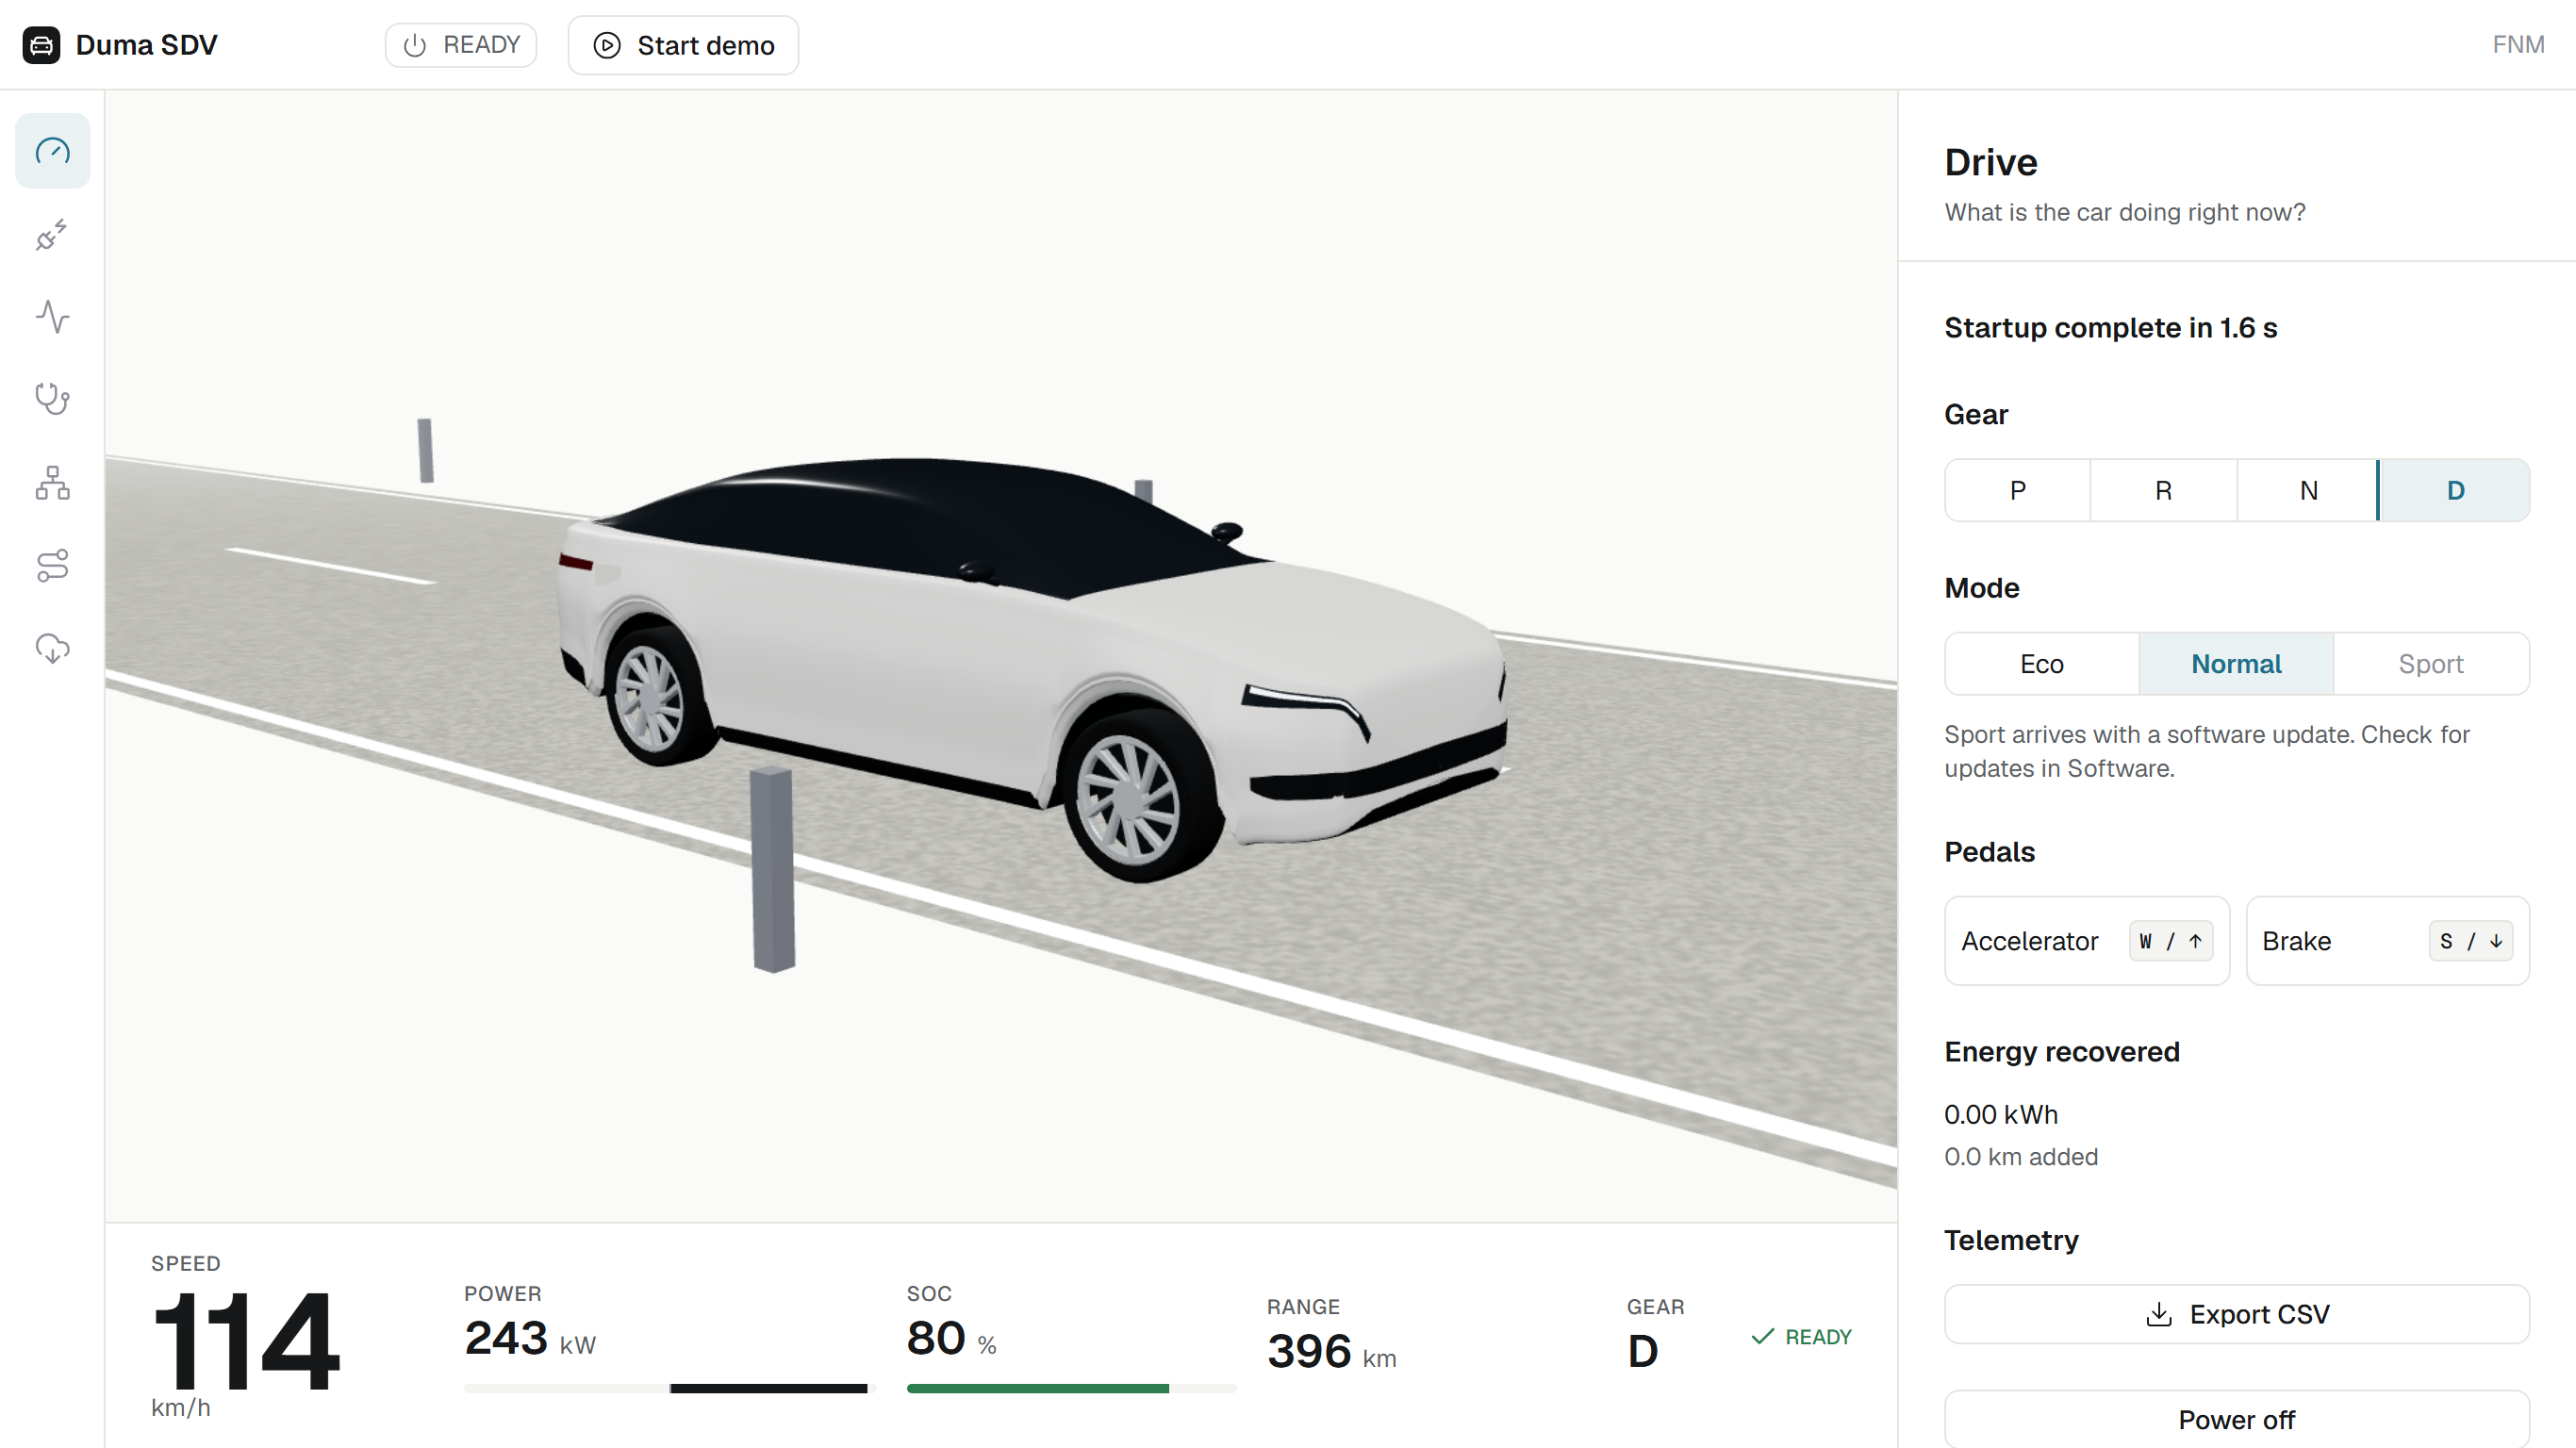
\includegraphics[width=\linewidth]{ui-drive}
\caption{Drive at 114\,km/h: the dashboard strip under the stage shows speed, power, SOC, range and gear, all from bus frames.}
\end{subfigure}\hfill
\begin{subfigure}[t]{0.49\textwidth}\centering
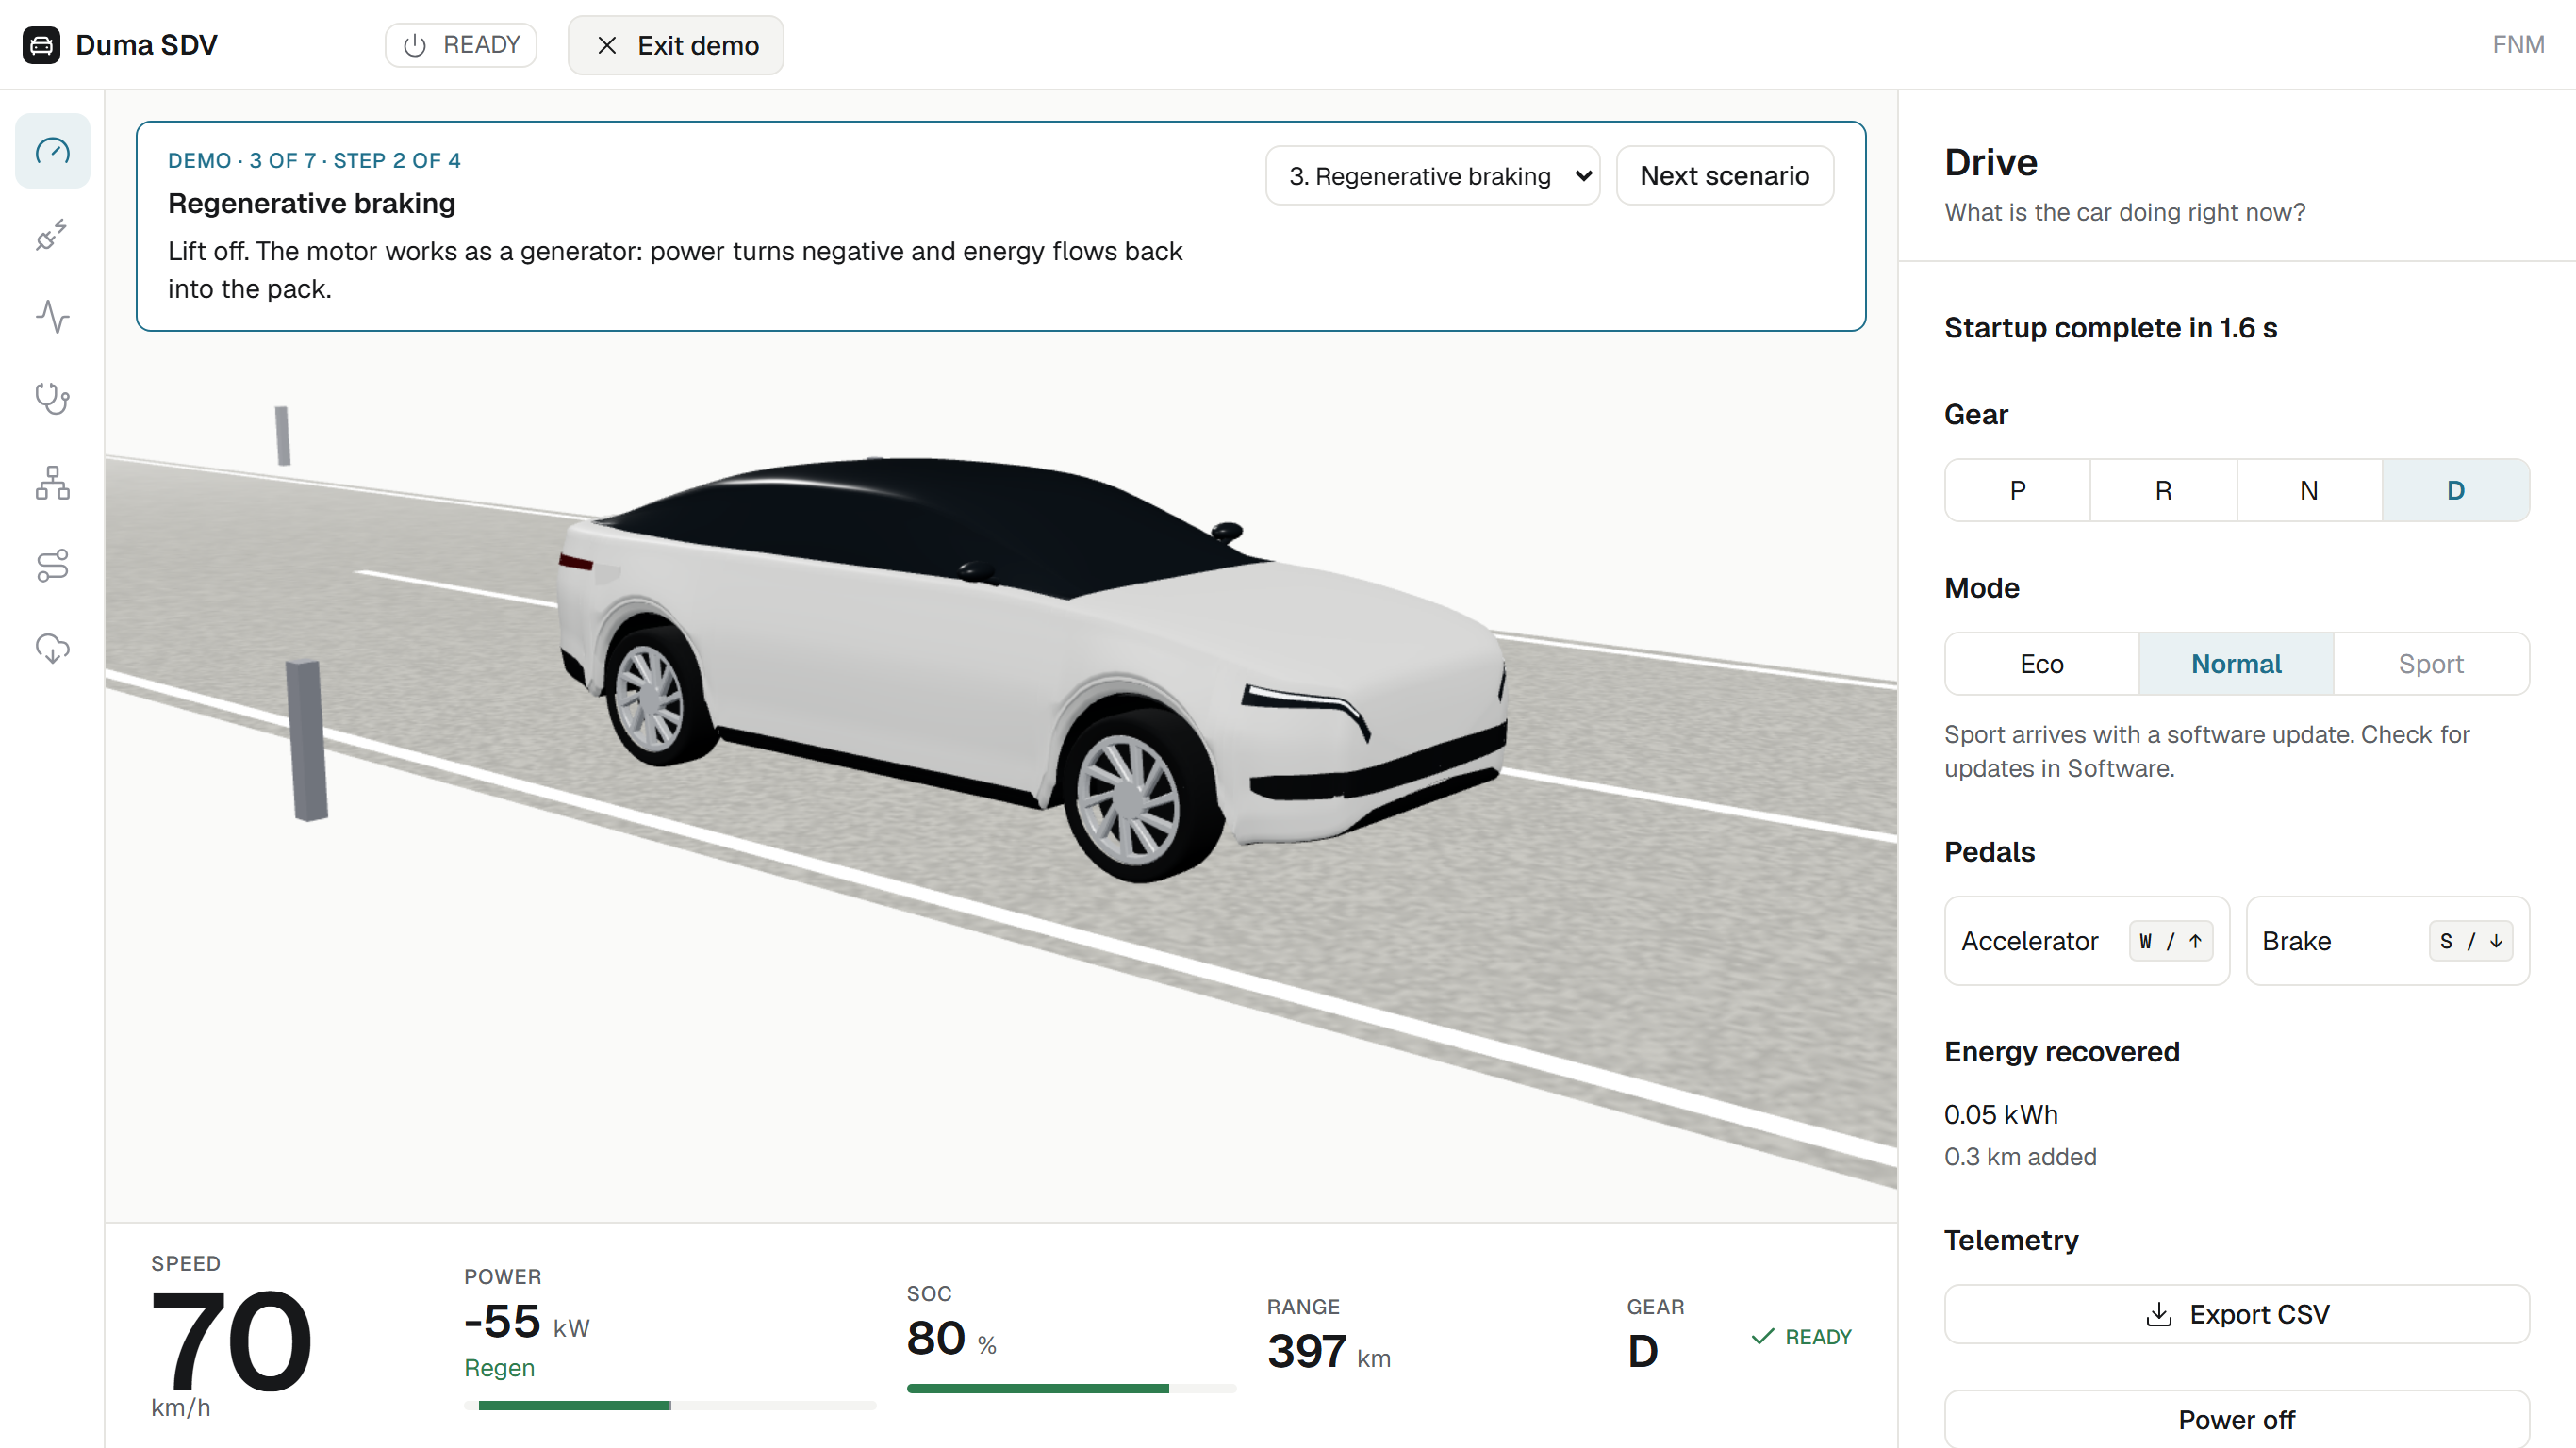
\includegraphics[width=\linewidth]{ui-demo}
\caption{Guided demo, Regen scenario: the caption bar over the stage explains the negative power on the dashboard.}
\end{subfigure}\par\medskip
\begin{subfigure}[t]{0.49\textwidth}\centering
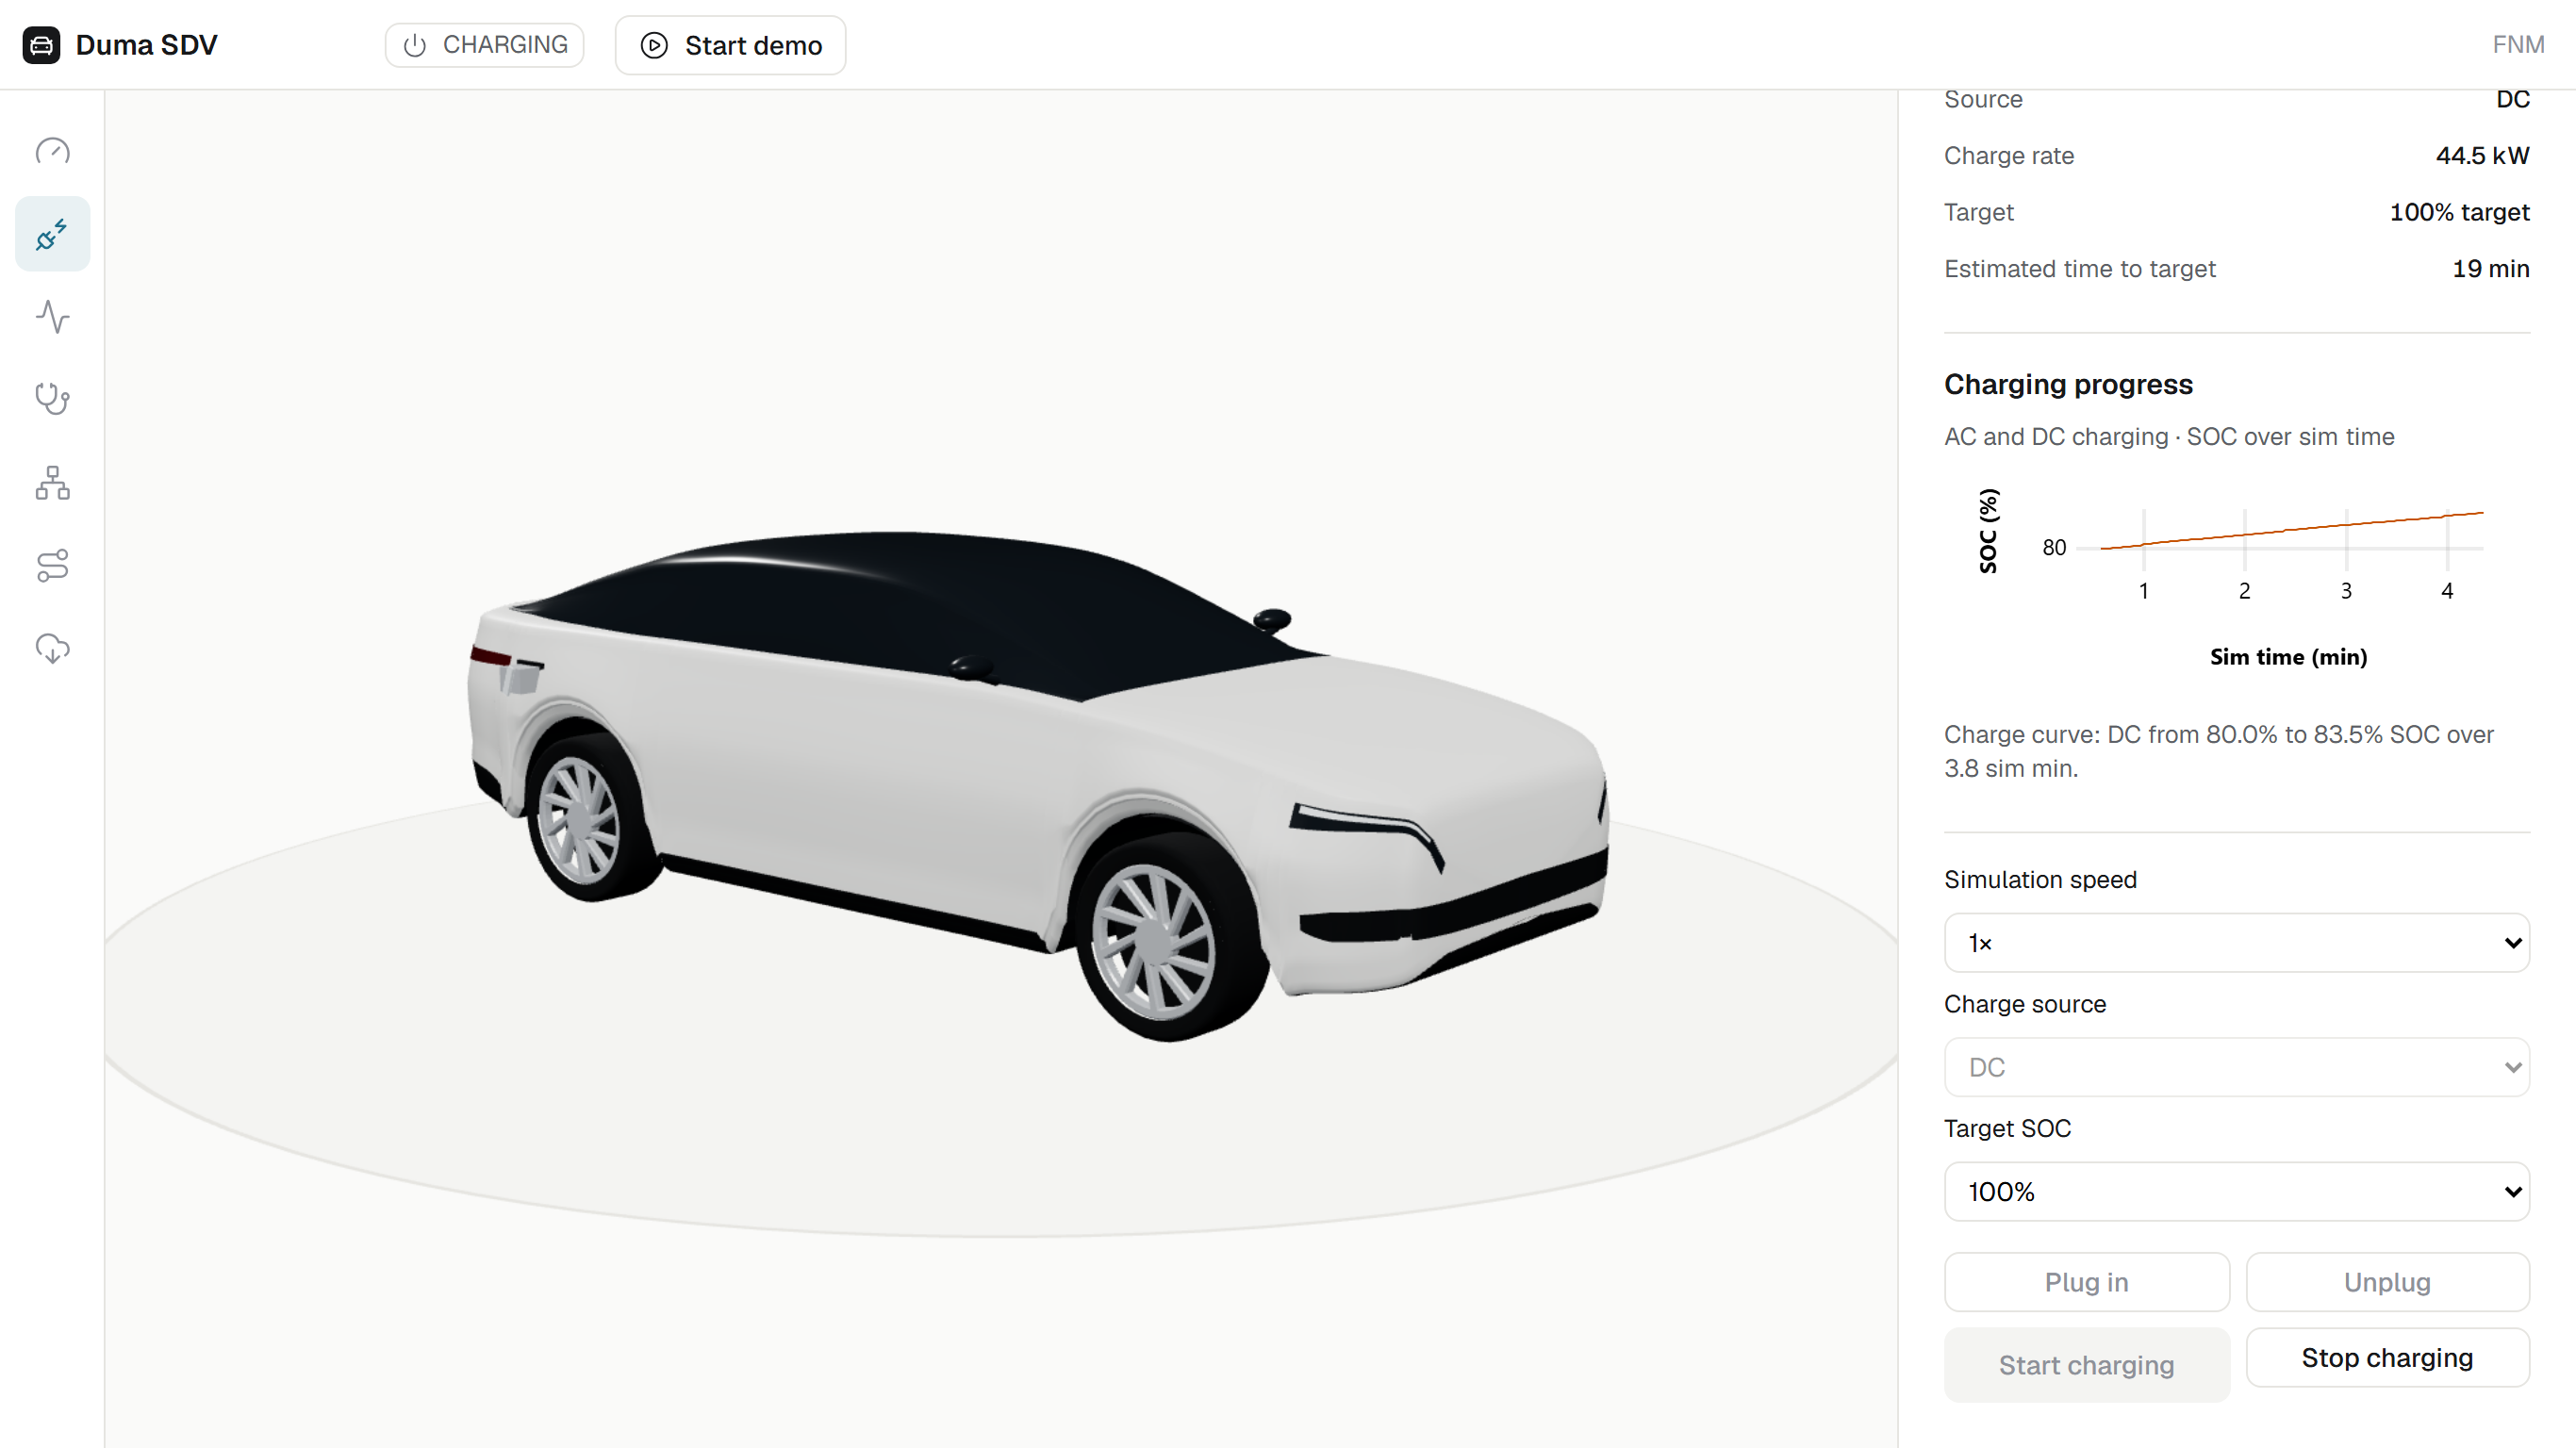
\includegraphics[width=\linewidth]{ui-charge}
\caption{Charge: a DC session at 120$\times$ time, with the charge curve and time to target.}
\end{subfigure}\hfill
\begin{subfigure}[t]{0.49\textwidth}\centering
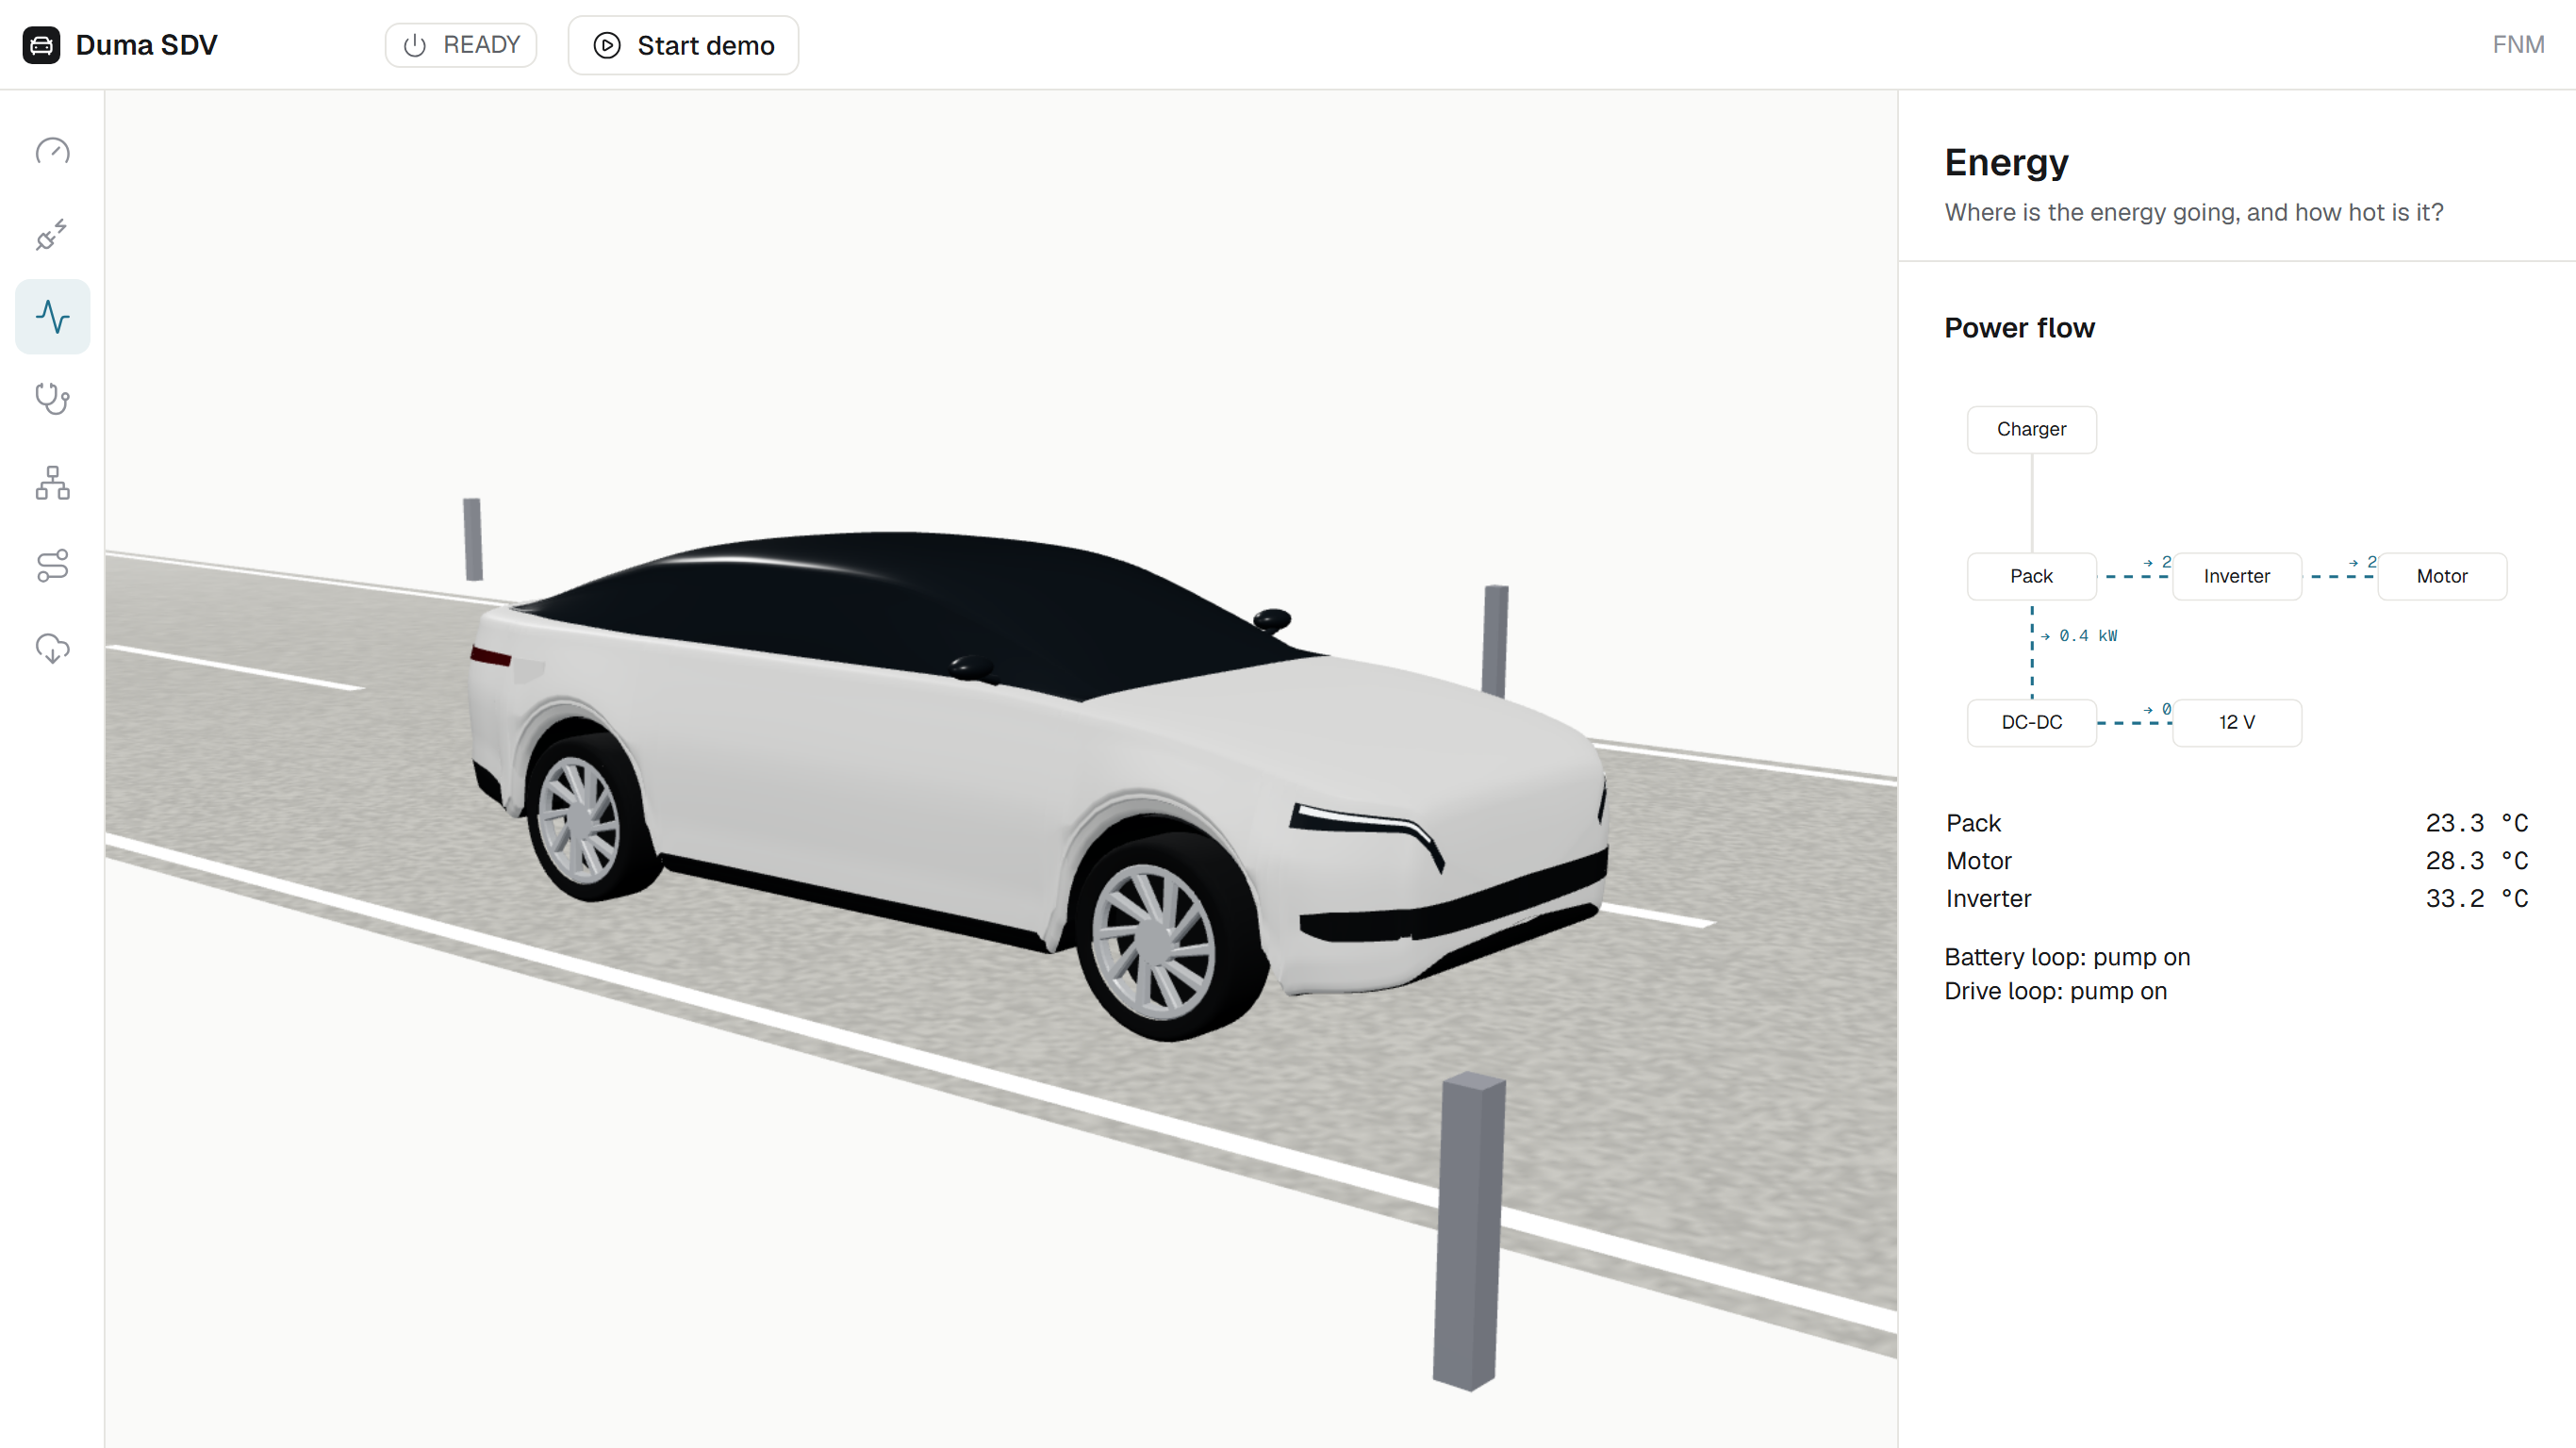
\includegraphics[width=\linewidth]{ui-energy}
\caption{Energy: live power flow between pack, inverter, motor, charger and DC-DC, with temperatures and coolant pumps.}
\end{subfigure}\par\medskip
\begin{subfigure}[t]{0.49\textwidth}\centering
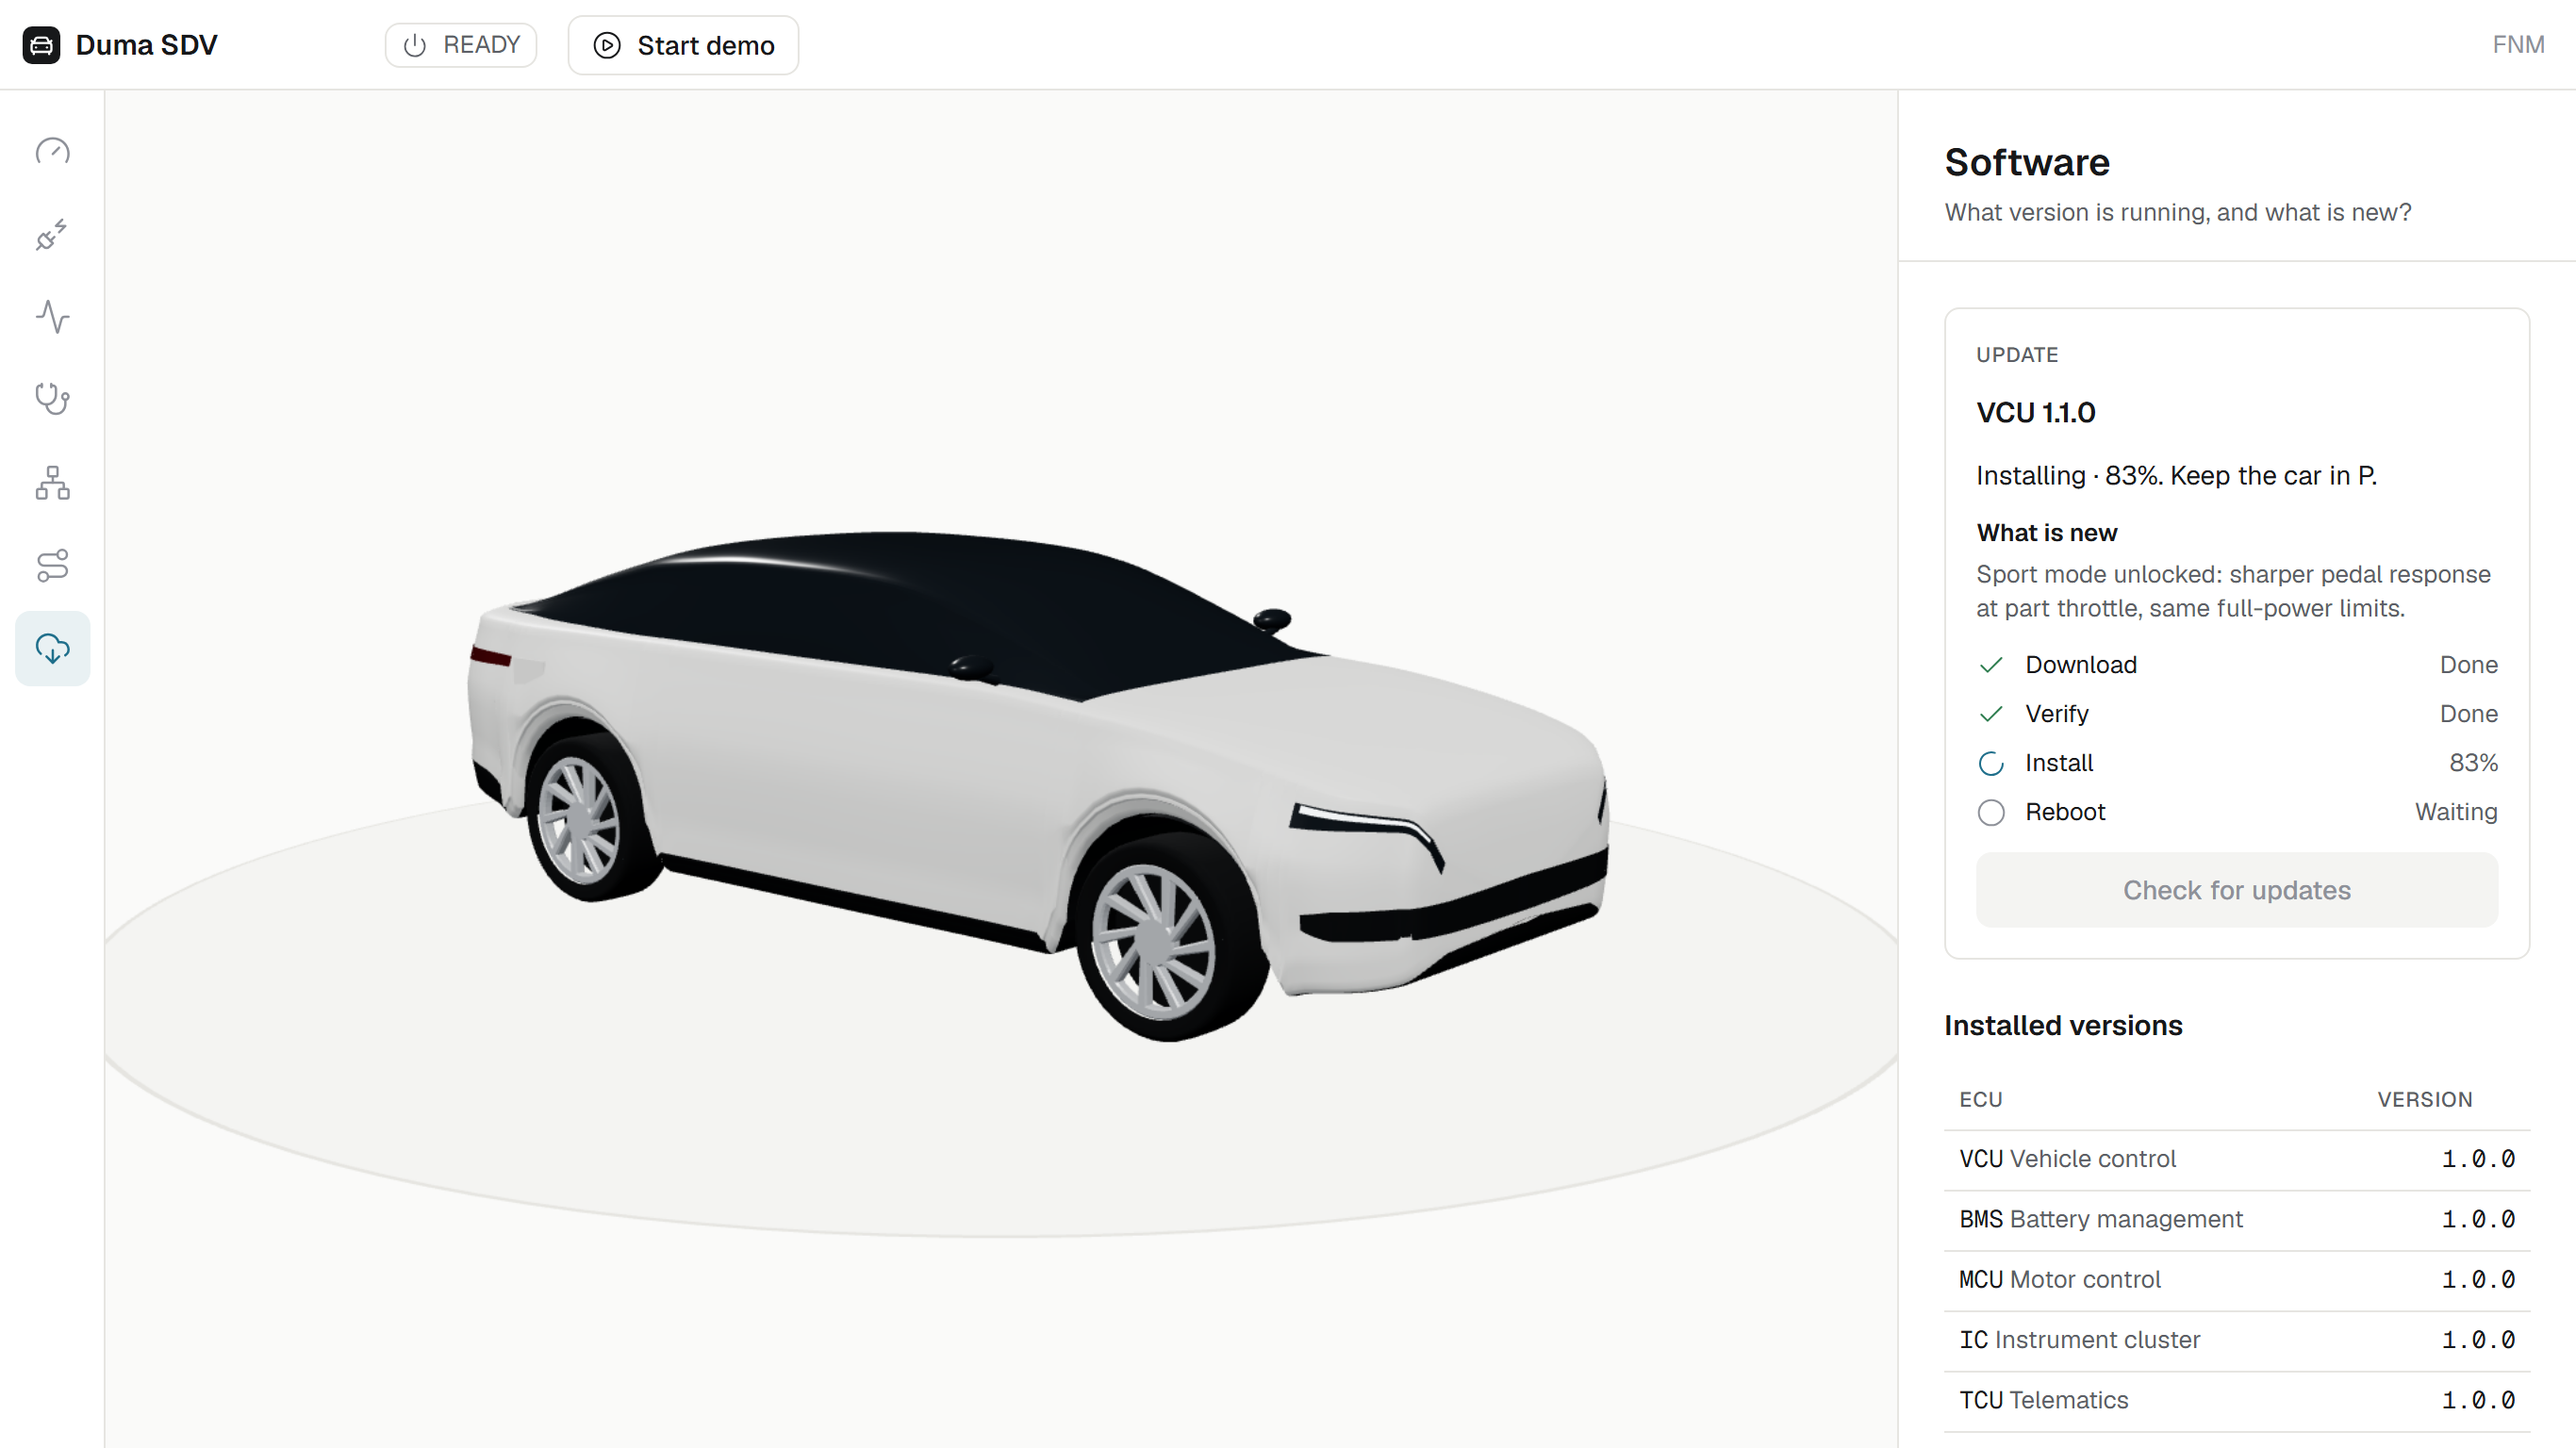
\includegraphics[width=\linewidth]{ui-software}
\caption{Software: the update is written to the VCU's inactive bank while the car stays in P.}
\end{subfigure}\hfill
\begin{subfigure}[t]{0.49\textwidth}\centering
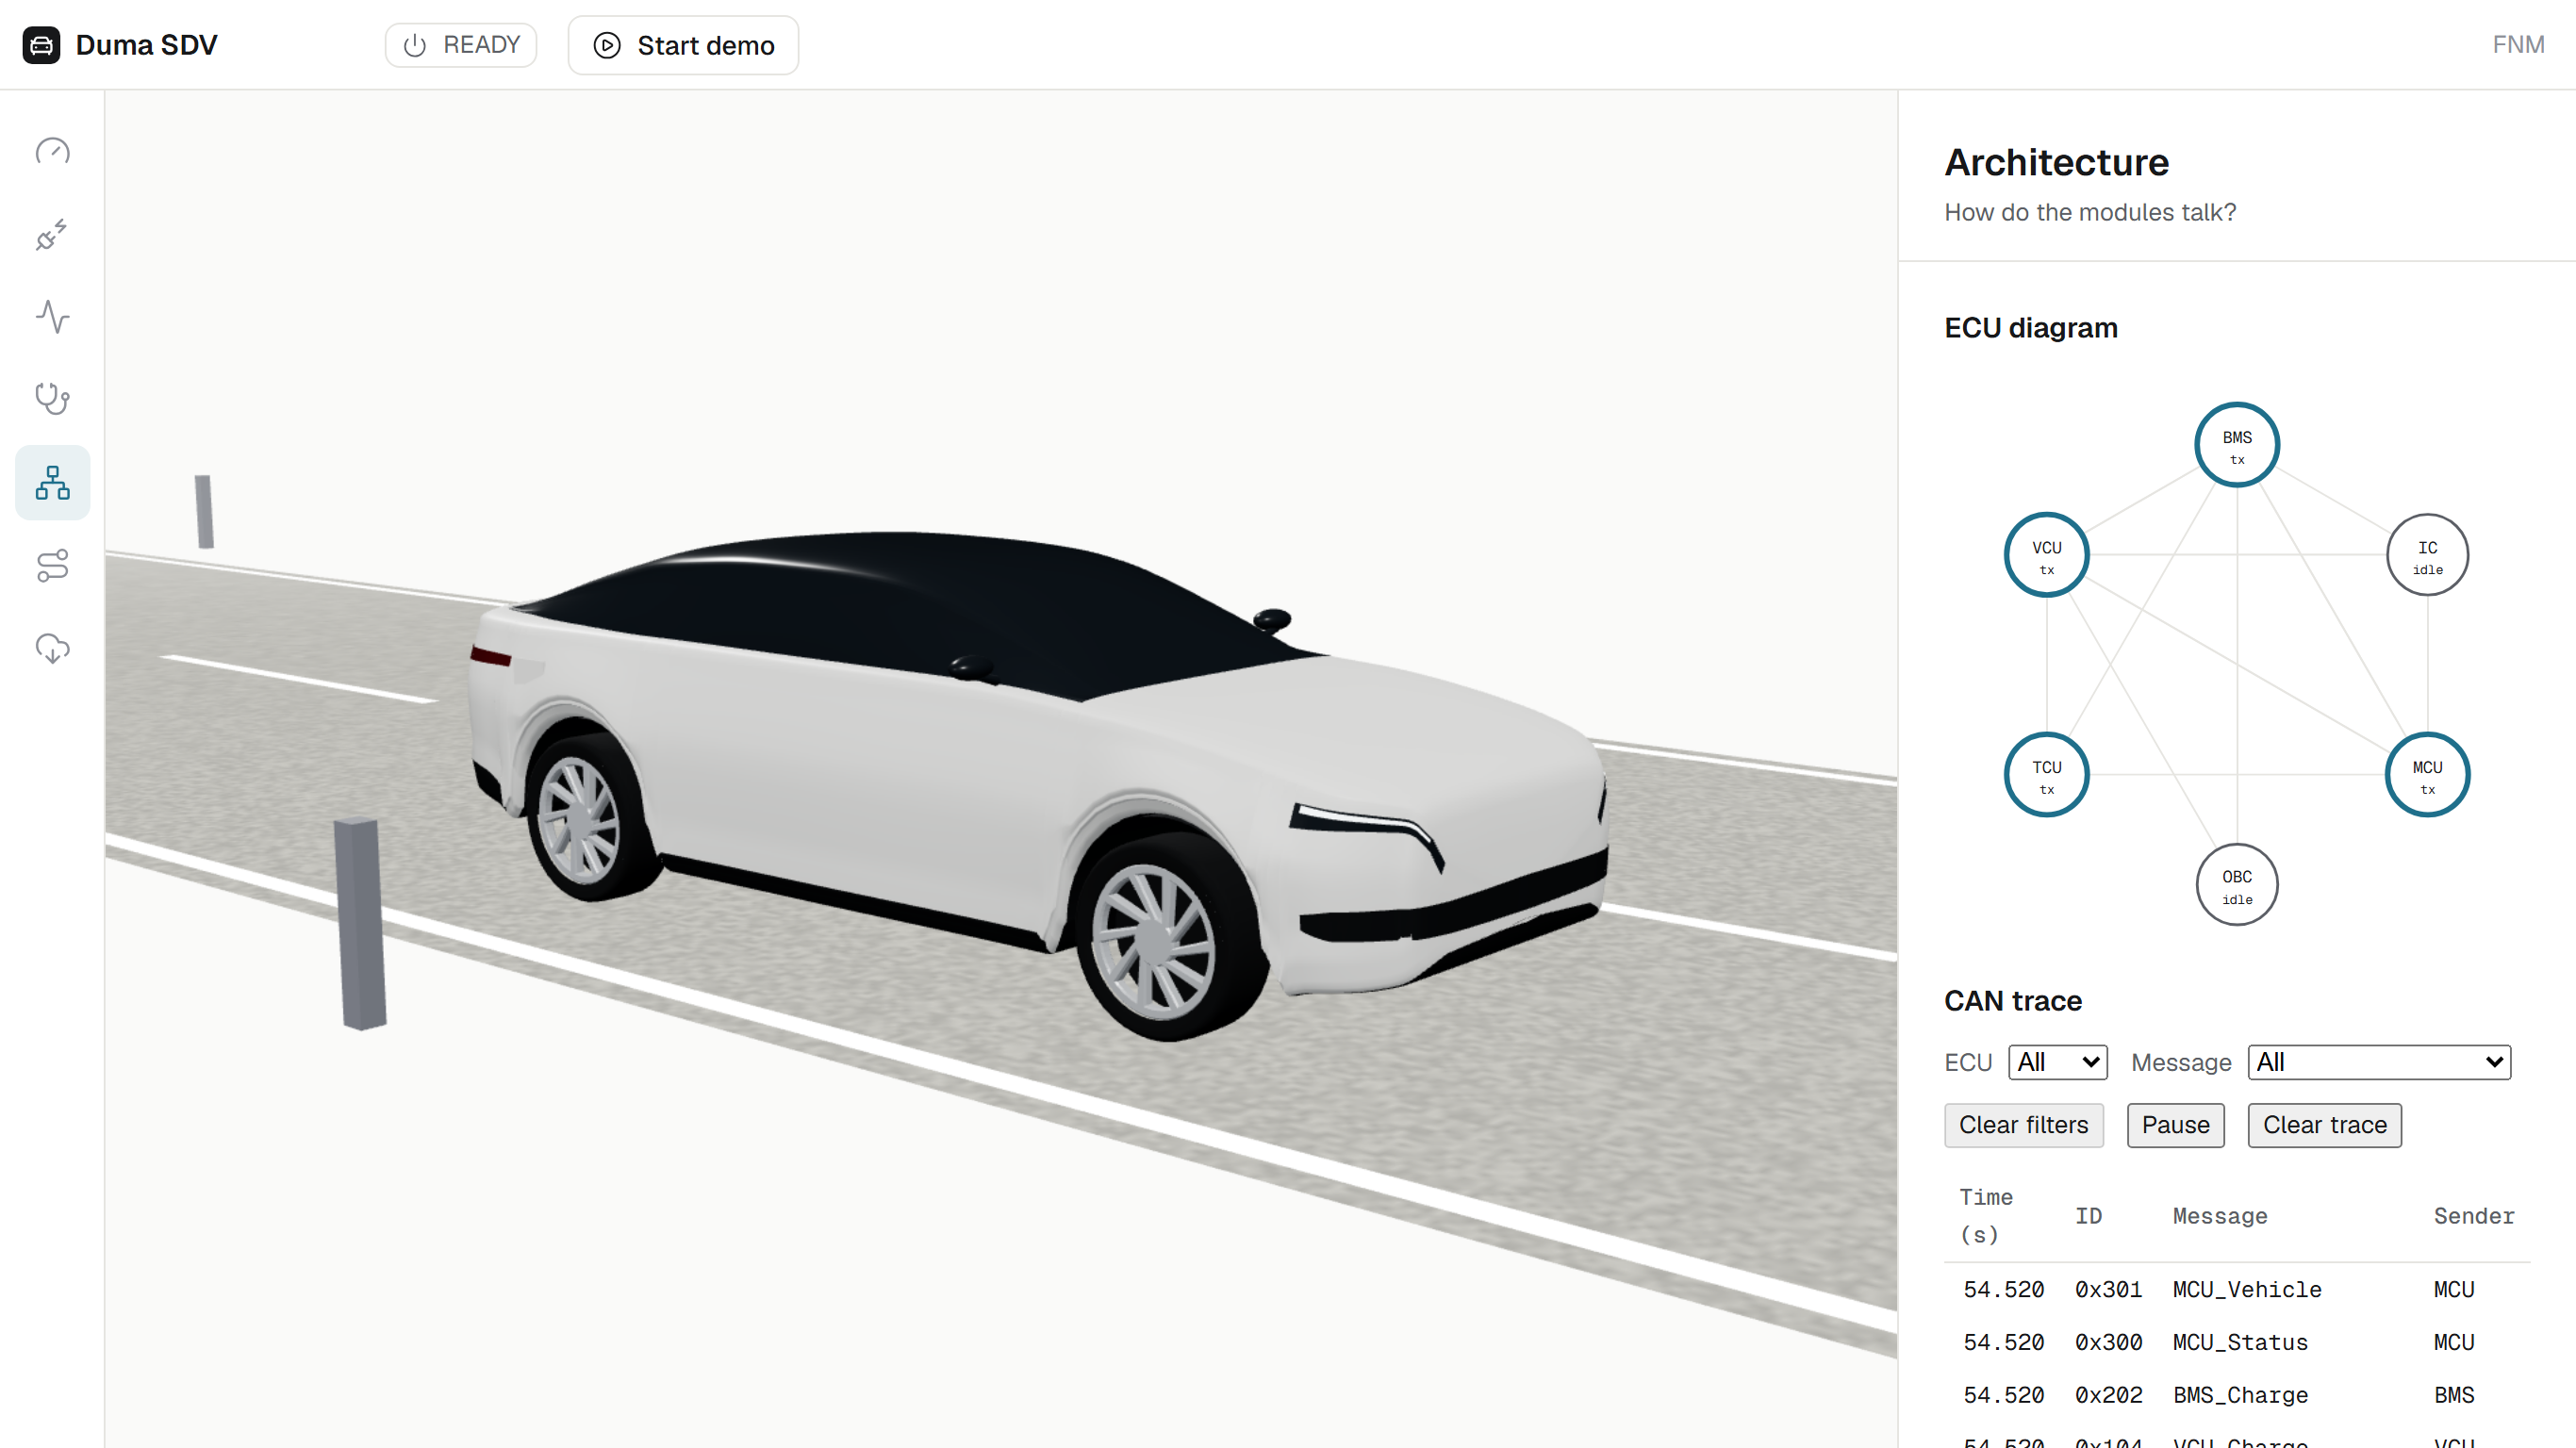
\includegraphics[width=\linewidth]{ui-architecture}
\caption{Architecture while driving: the 3D stage on the left and the ECU diagram on the right.}
\end{subfigure}
\caption{\textbf{The application at 1366$\times$768}, captured from the production build. A left rail switches views, the 3D stage fills the middle, and the right panel answers the view's one question.}
\label{fig:ui}
\end{figure}

The guided demo plays all six scenarios from one button. Each scenario is a script of steps with a caption, a view, a time scale, the inputs to apply and the condition that ends the step. The demo drives the car only through the same inputs a driver uses. Each scenario starts from a fresh simulation prepared headlessly, so any scenario can be played on its own, and a step that does not finish within its timeout stops the demo with an error instead of hanging. The production build is a progressive web app whose service worker caches the whole application, so it runs at a venue with no network.

% ==============================================================================
\section{Vehicle model and calibration}
% ==============================================================================

The longitudinal model integrates tractive force against aerodynamic drag, rolling resistance and grade, with a rotational mass factor~\cite{gillespie1992}. Motor and inverter loss is a four-term map in torque and speed. The pack is \ParCells{} LFP cells in series (\ParPackV\,V nominal, \ParPackKwh\,kWh usable) with an SOC-dependent open-circuit voltage and a series resistance. Published figures of the reference car set the official parameters (Table~\ref{tab:params}). Parameters the reference car does not publish, such as losses, internal resistance and thermal masses, are estimates, each marked in the code and recorded in a decision record. When a reference test missed, only the estimates were tuned, never the official figures or the tolerances.

\begin{table}[!htbp]
\caption{\textbf{Main vehicle parameters.} Official figures of the reference car except where marked.}
\label{tab:params}
\centering\small
\begin{tabular}{@{}lr@{\qquad}lr@{}}
\toprule
Motor peak power & \ParMotorKw\,kW & Test mass & \ParTestMass\,kg \\
Motor peak torque & \ParMotorNm\,N\,m & Drag coefficient & \ParCd \\
Reduction ratio & \ParRatio & Frontal area (estimate) & \ParArea\,m$^2$ \\
Usable pack energy & \ParPackKwh\,kWh & Rolling resistance (estimate) & \ParCrr \\
Pack nominal voltage & \ParPackV\,V & AC / DC peak charge & \ParObcKw\,/\,\ParDcKw\,kW \\
\bottomrule
\end{tabular}
\end{table}

\begin{table}[!htbp]
\caption{\textbf{Reference tests.} Each is an automated test with a fixed $\pm 10\,\%$ window around the reference car's published figure.}
\label{tab:reference}
\centering\small
\begin{tabular}{@{}lrrr@{}}
\toprule
Figure & Target & Window & Simulated \\
\midrule
0--100\,km/h & 5.9\,s & 5.31--6.49\,s & \ResZeroHundred\,s \\
Range at a steady 100\,km/h (100--0\,\% usable) & 510\,km & 459--561\,km & \ResRange\,km \\
DC charge 10--80\,\% & 37\,min & 33.3--40.7\,min & \ResDcMin\,min \\
\bottomrule
\end{tabular}
\end{table}

Table~\ref{tab:reference} shows the three reference tests. Consumption at a steady 100\,km/h is \ResRangeWhKm\,Wh/km, and \ResAnchorWhKm\,Wh/km at 110\,km/h, inside the 172--190\,Wh/km band we used as the calibration anchor. The DC charge peaks at \ResDcPeakKw\,kW. An AC charge over the same window takes \ResAcHours\,h, limited by the on-board charger.

% ==============================================================================
\section{Scenario results}
% ==============================================================================

\paragraph{Acceleration.} Figure~\ref{fig:accel} shows a full-pedal start. Torque is flat at \ParMotorNm\,N\,m up to base speed, after which power is held near its limit and torque falls. The run reaches 100\,km/h in \ResZeroHundred\,s. Pack power exceeds shaft power by the motor and inverter losses.

\begin{figure}[!htbp]
\centering
\begin{subfigure}[t]{0.49\textwidth}
\begin{tikzpicture}
\begin{axis}[xlabel={Time (s)}, ylabel={Speed (km/h)}, xmin=0, xmax=10, ymin=0, legend pos=south east]
\addplot[dblue] table[x=t_s, y=speed_kmh, col sep=comma] {data/accel.csv};
\draw[dgrey, densely dotted] (axis cs:\ResZeroHundred,0) -- (axis cs:\ResZeroHundred,100) -- (axis cs:0,100);
\legend{speed}
\end{axis}
\end{tikzpicture}
\caption{Speed; dotted lines mark 100\,km/h.}
\end{subfigure}\hfill
\begin{subfigure}[t]{0.49\textwidth}
\begin{tikzpicture}
\begin{axis}[xlabel={Time (s)}, ylabel={Power (kW)}, xmin=0, xmax=10, ymin=0, legend pos=south east]
\addplot[dorange] table[x=t_s, y=pack_kw, col sep=comma] {data/accel.csv};
\addplot[dblue] table[x=t_s, y=shaft_kw, col sep=comma] {data/accel.csv};
\legend{battery, motor shaft}
\end{axis}
\end{tikzpicture}
\caption{Battery and shaft power.}
\end{subfigure}
\caption{\textbf{Full-pedal acceleration from rest in Normal.}}
\label{fig:accel}
\end{figure}

\paragraph{Regenerative braking.} From 100\,km/h the driver lifts off for \ResRegenLiftS\,s and then holds the brake at 30\,\% until the car stops, \ResRegenBrakeS\,s later (Figure~\ref{fig:regen}). At \ResRegenSocPct\,\% SOC the BMS allows \ResRegenAllowKw\,kW of charge, so regen stays at that allowance (peak \ResRegenPeakKw\,kW at the pack) and the friction brakes supply the rest of the pedal's demand. Of the \ResRegenKineticKj\,kJ of kinetic energy at the start, \ResRegenPackKj\,kJ (\ResRegenShare\,\%) reaches the pack; the rest goes to road load, drivetrain losses and the friction brakes at low speed. The trip tracker shows \ResRegenRecoveredWh\,Wh recovered.

\begin{figure}[!htbp]
\centering
\begin{tikzpicture}
\begin{axis}[xlabel={Time (s)}, ylabel={Speed (km/h), power (kW)}, xmin=0, ymin=-80, ymax=120, legend pos=north east]
\addplot[dblue] table[x=t_s, y=speed_kmh, col sep=comma] {data/regen.csv};
\addplot[dorange] table[x=t_s, y=pack_kw, col sep=comma] {data/regen.csv};
\draw[dgrey, densely dotted] (axis cs:\ResRegenLiftS,-80) -- (axis cs:\ResRegenLiftS,110) node[pos=0.98, anchor=north west, font=\tiny, text=dgrey] {brake};
\legend{speed (km/h), battery power (kW)}
\end{axis}
\end{tikzpicture}
\caption{\textbf{Regenerative stop from 100\,km/h.} Battery power turns negative on lift-off and is held at the BMS charge allowance through the braking, while the friction brakes take the remaining demand. Regen fades out below 5\,m/s and the friction brakes finish the stop.}
\label{fig:regen}
\end{figure}

\paragraph{Charging.} Figure~\ref{fig:charge} compares the two sources. The DC charge starts at the charger's peak and tapers as the pack fills; the AC charge is flat at the on-board charger's limit less conversion loss.

\begin{figure}[!htbp]
\centering
\begin{subfigure}[t]{0.49\textwidth}
\begin{tikzpicture}
\begin{axis}[xlabel={SOC (\%)}, ylabel={Charger input (kW)}, xmin=10, xmax=80, ymin=0, legend pos=north east]
\addplot[dorange] table[x=soc_pct, y=input_kw, col sep=comma] {data/dc_charge.csv};
\addplot[dblue] table[x=soc_pct, y=input_kw, col sep=comma] {data/ac_charge.csv};
\legend{DC, AC}
\end{axis}
\end{tikzpicture}
\caption{Charging power against SOC.}
\end{subfigure}\hfill
\begin{subfigure}[t]{0.49\textwidth}
\begin{tikzpicture}
\begin{axis}[xlabel={Time (min)}, ylabel={SOC (\%)}, xmin=0, xmax=40, ymin=0, ymax=100, legend pos=south east]
\addplot[dorange] table[x=t_min, y=soc_pct, col sep=comma] {data/dc_charge.csv};
\legend{DC}
\end{axis}
\end{tikzpicture}
\caption{DC charge, 10--80\,\% in \ResDcMin\,min.}
\end{subfigure}
\caption{\textbf{AC and DC charging from 10\,\% to 80\,\% SOC.} The AC charge takes \ResAcHours\,h.}
\label{fig:charge}
\end{figure}

\paragraph{Drive cycles.} A speed-tracking driver model follows the Low and Extra High phases of the WLTC Class~3 cycle~\cite{unece_gtr15} using only the pedal inputs (Figure~\ref{fig:cycles}). In Normal the Urban phase covers \CycUrbanKm\,km on \CycUrbanKwh\,kWh and the Highway phase \CycHighwayKm\,km on \CycHighwayKwh\,kWh. The modes differ little in energy (Table~\ref{tab:modes}): on a fixed speed trace the wheel energy is the same, and Eco's stronger lift-off regen adds round-trip battery loss. The modes change how the car responds, not how much energy the trip needs. Over the Highway phase the motor warms to \CycHighwayMotorMaxC\,$^\circ$C while the pack, with its large heat capacity, stays at \CycHighwayPackMaxC\,$^\circ$C.

\begin{figure}[!htbp]
\centering
\begin{subfigure}[t]{0.49\textwidth}
\begin{tikzpicture}
\begin{axis}[xlabel={Time (s)}, ylabel={Speed (km/h)}, xmin=0, xmax=\CycUrbanDurS, ymin=0, legend pos=north west]
\addplot[dgrey, dashed] table[x=t_s, y=target_kmh, col sep=comma] {data/cycle_urban.csv};
\addplot[dblue] table[x=t_s, y=speed_kmh, col sep=comma] {data/cycle_urban.csv};
\legend{target, speed}
\end{axis}
\end{tikzpicture}
\caption{Urban (WLTC Low phase).}
\end{subfigure}\hfill
\begin{subfigure}[t]{0.49\textwidth}
\begin{tikzpicture}
\begin{axis}[xlabel={Time (s)}, ylabel={Battery power (kW)}, xmin=0, xmax=\CycHighwayDurS, legend pos=south west]
\addplot[dorange] table[x=t_s, y=battery_kw, col sep=comma] {data/cycle_highway.csv};
\legend{battery power}
\end{axis}
\end{tikzpicture}
\caption{Highway (WLTC Extra High phase).}
\end{subfigure}
\caption{\textbf{Drive cycles in Normal.} The driver tracks the target within $\pm 2$\,km/h for at least 98\,\% of samples. Negative battery power is regen; the spikes near the end of the Highway phase are the driver model pulsing the brake on the final deceleration, sampled once a second.}
\label{fig:cycles}
\end{figure}

\paragraph{Fault response.} Two identical full-pedal runs start from rest; in one, a cell over-temperature fault is injected at 2\,s and restored at 5\,s (Figure~\ref{fig:fault}). The chain is visible on the bus. The BMS sends the DTC and a halved discharge allowance of \FaultLimitKw\,kW \FaultDtcMs\,ms after injection. The IC shows the warning after \FaultWarningMs\,ms and the VCU's drive decision names the cause after \FaultDecisionMs\,ms. Battery power follows the allowance: at \FaultCompareS\,s the faulted car draws \FaultDeratedKw\,kW against \FaultHealthyKw\,kW for the healthy one. Building this figure exposed a defect: the VCU had applied the discharge limit to shaft power, so losses pushed battery power about 8\,\% past the limit. It now applies the limit at the battery, and a test holds it there.

\begin{figure}[!htbp]
\centering
\begin{tikzpicture}
\begin{axis}[xlabel={Time (s)}, ylabel={Battery power (kW)}, xmin=0, xmax=7, ymin=0, ymax=300, legend pos=south east]
\fill[warn, opacity=0.10] (axis cs:2,0) rectangle (axis cs:5,300);
\addplot[dgrey, dashed] table[x=t_s, y=healthy_kw, col sep=comma] {data/fault.csv};
\addplot[dorange] table[x=t_s, y=pack_kw, col sep=comma] {data/fault.csv};
\draw[fault, densely dotted] (axis cs:2,\FaultLimitKw) -- (axis cs:5,\FaultLimitKw) node[pos=0.5, anchor=south, font=\tiny, text=fault] {BMS allowance \FaultLimitKw\,kW};
\legend{healthy, with fault}
\end{axis}
\end{tikzpicture}
\caption{\textbf{Cell over-temperature while accelerating.} The shaded band is the fault. Power is capped at the BMS allowance and returns when the condition clears; the DTC stays stored until cleared.}
\label{fig:fault}
\end{figure}

\paragraph{OTA update.} The update completes in \OtaReadyS\,s from the first click (Table~\ref{tab:ota}), of which the restart takes \OtaRestartS\,s. The trace shows the TCU's progress, the power-down, and the new boot frame.

% ==============================================================================
\section{Verification}
% ==============================================================================

The project was built in phases from a written brief. Each phase had requirements, validation checks and small tickets, and each ticket had to pass typecheck, lint, the unit tests, the production build and the browser tests before it was committed. Decisions that the brief did not settle are recorded in seventeen decision records.

\begin{itemize}
  \item \textbf{Unit and simulation tests} (Vitest, 380 tests): bus timing, startup and its failure paths, gear interlocks, pedal maps and mode ramps, regen blending, AC and DC charging, faults and DTCs, thermal balance, drive cycles, telemetry, the OTA client and firmware banks, the guided demo scripts played headlessly, every view, and the reference tests of Table~\ref{tab:reference}.
  \item \textbf{Browser tests} (Playwright, 27 tests at 1366$\times$768): every scenario unaided and again from the guided demo, the architecture trace, CSV export, and an offline reload served by the service worker.
  \item \textbf{Determinism}: identical inputs give identical snapshots and bus traces.
\end{itemize}

Of the brief's definition of done, the scenario, physics, offline and paper items are met and verified by the tests above. The public link is deferred by decision, and the build is ready for any static host. The review of every view against the design contract is a manual check.

% ==============================================================================
\section{Limitations}
% ==============================================================================

The model is a teaching and review tool, not a validated engineering simulation. The thermal model has one mass per component and two coolant loops. The battery has one resistance and no transient dynamics. The bus has no bit timing, arbitration or error frames. Many parameters are estimates, marked as such. The OTA verification step always passes; a real one would check a signature chain and roll back after a failed boot. The car drives on a rolling road with no steering or lateral dynamics.

% ==============================================================================
\section{Conclusion}
% ==============================================================================

\sdv{} turns an SDV software architecture into something a judge can operate. Six ECUs coordinate only through a catalogued bus, over physics that reproduces the reference car's acceleration, range and charge time within $\pm 10\,\%$. The fault, charging and update flows can be traced message by message. Because the core is deterministic and free of the user interface, the same code serves the live demo, the automated tests and every figure in this paper. Making the paper's figures from the simulator also exposed a real defect, the discharge limit applied at the shaft instead of the battery, which is now fixed and guarded by a test.

\bibliographystyle{plainnat}
\bibliography{references}

\end{document}
